\documentclass[10pt,a4paper]{article}
\usepackage[utf8]{inputenc}
\usepackage{amsmath}
\usepackage{adjustbox}
\usepackage{amsfonts}
\usepackage{amssymb}
\usepackage{graphicx}
\usepackage{subcaption}
\graphicspath{ {./graphics/} }
\usepackage[colorlinks]{hyperref}
\usepackage{wrapfig}
\usepackage{float}
\usepackage{svg}
\usepackage[
backend=biber,
style=numeric,
sorting=ynt
]{biblatex}
\addbibresource{6D-Ae-report.bib}
\newcommand{\R}{\mathbb{R}}
\usepackage{blindtext}
\usepackage{xspace}
\usepackage{tikz}
\usepackage{pgf}
\usetikzlibrary{arrows,arrows.meta,shapes,shapes.multipart,shapes.geometric,shapes.misc,calc,positioning,decorations.pathreplacing,fit,backgrounds,positioning,calc}

\newcommand{\rot}{\ensuremath{\text{rot}\xspace}}
\newcommand{\trans}{\ensuremath{\text{trans}\xspace}}
\newcommand{\loss}{\ensuremath{\mathcal{L}_2}}


\begin{document}
  % Keine Seitenzahlen im Vorspann
  \pagestyle{empty}

  % Titelblatt der Arbeit
  \begin{titlepage}


 \begin{center} 
	{\Large\textbf{ 
		6D Pose Autoencoder
	}}
    \vspace{1cm}
    
    Project report Reconstructing and Understanding the 3D World\\
    at the IWR Institute in Heidelberg\\
    \vspace{5cm}
    submitted by\\
    \vspace{0.5cm}
	{\large\textbf{Till Bungert and Carsten Lüth}\\}
	\vspace{5cm}
	under the supervision of \\
	\vspace{0.5cm}
	{\large\textbf{Prof. Dr. Carsten Rother}\\}
	and\\
	{\large\textbf{Siva Karthik Mustikovela}\\}


    \vspace{3cm}
	{\Large\textbf{2018}}
	

	

  \end{center}
\end{titlepage}


  % Inhaltsverzeichnis
  \tableofcontents

\newpage

  % Ab sofort Seitenzahlen in der Kopfzeile anzeigen
  \pagestyle{headings}

\section{Introduction}\label{Introduction}
The determination of 6D poses for known objects is a very important subject for robotics and augmented reality. For example in robotics it is crucial to have an accurate understanding of the position of an object to interact with it in a meaningful way. Almost the same applies to augmented reality because to enhance any object by rendering information on its visible surface it is important to know the position of the said object.\\
There are many different ways to determine the 6D-Pose of a known object but in this work we will concentrate on a method which is based on the Augmented Autoencoder as designed by Martin Sundermeier et al. \cite{3D_Orientation_Learning}. This approach only uses RGB Images and does not require a big amount of labelled data to be trained because the autoencoder is tasked to reconstruct its input and not to predict the rotation and translation directly. This implicit learning makes it very robust against symmetries. Also in their paper they show that it can be fully trained on artificial generated images and also able to generalize to real images.\\
The general goal of this work is to use the augmented autoencoder to disentangle the rotation and translation information in the latent space with a novel training scheme as well as to give an theoretical motivation for the rotation learning of the network which gets backed up by our experiments. Due to the training schedule the training is self-supervised and completely conducted on rendered images.\\
All of our experiments are conducted on rendered data and also validated on rendered images. To render the images we used the open source renderer GLUMPY \cite{GLUMPY} based on Numpy and OpenGL. \\  




\newpage

\section{Methods}\label{Methods}
In the following section we focus on the novel 6D-Autoencoder which is a new interpretation of the Augmented Autoencoder (AAE), introduced by Martin Sundermeier et al. \cite{3D_Orientation_Learning}. First we introduce the concept of invariant latent space representations of an Autoencoder via objective functions and then present a method to get the 6D-Pose based on the latent space representation.

\subsection{Autoencoder}\label{Autoencoder}
The original Autoencoder is a technique to map a high dimensional input ($x \in \mathbb{R}^N$), such as image or audio data, into a lower dimensional representation ($z \in \mathbb{R}^D$) ($D << N$) while maintaining the important information of its input. To achieve this the model which consists of an Encoder $\varphi$ and Decoder $\phi$ is tasked to reconstruct its input after passing it through a low dimensional bottleneck ($z$), where each of them is a general function approximator (neural network), resulting in the following objective function:
\begin{equation}
\min_{\varphi, \phi} L_{\text{rec}}(x, \phi(\varphi(x)))
\end{equation}
$L_{\text{rec}}$ can be any arbitrary distance metric on $\mathbb{R}^N$. 
A specialized form of the Autoencoder is the  Denoising Autoencoder. For this type of Autoencoder the input $x$ gets pertubed with random noise $\tilde{x} = f_{\text{noise}}(x) =x + \epsilon$ with $\epsilon \sim \mathbb{P}_{\epsilon}$ while being tasked to reconstruct the unpertubed $x$. This results in the following objective function:
\begin{equation}
\min_{\varphi, \phi} L_{\text{rec}}(x, \phi(\varphi(f_{\text{noise}}(x) )))
\end{equation}
The trained model can be used to reconstruct unpertubed test images. But how is the latent space effected by this training schedule?
This question leads to the core assumption to create the AAE which gets motivated by a later experiment.
\paragraph{Hypothesis 1} To optimally reconstruct the unpertubed $x$ for the previously unseen test data the encoder should get in theory invariant to the pertubation. Meaning: Encoded Latent space representation of the input is invariant against the perturbation.\\
\paragraph{Regularized Autoencoder}
The regularized Autoencoder as described in the `Deep Learning Book' by Goodfellow  \cite{Goodfellow} is defined by an additional loss or part of the objective function which is solely effected by the latent space representation. By adding this additional loss the latent space gains some desired properties such as a specific distribution with the Variational Autoencoder by using the KL-Divergence as latent loss.
Resulting objective function of a regularized Autoencoder:
\begin{equation}
\min_{\varphi, \phi} L_{\text{rec}}(x, \phi(\varphi(f(x) ))) + L_{\text{lat}}(\varphi(f(x)))
\end{equation}
$f$ can be any arbitrary augmentation or just the identity.

\subsection{6D Pose Autoencoder}\label{6D Pose Autoencoder}
\begin{figure}[htb]
    \centering
    \begin{tikzpicture}[
    coder/.style = {trapezium, trapezium angle=70, minimum width=20mm, draw, thick},
    trapezium stretches=true,
    vector/.style = {rectangle split, rounded corners=1mm, rectangle split
        parts=2, thick, draw, inner ysep=5mm, rectangle split part
    fill={lime!40, orange!40}},
    mat/.style = {inner sep=0mm, column sep=0mm,nodes=draw},
    img/.style = {inner sep=0, outer sep=-3mm},
    fat arrow/.style = {double arrow, thick, draw, anchor=mid, align=center,
    text depth=-0.5pt, text width = 1.5cm, text = black},
    node distance = 5mm
    ]
    \node [vector] (z) {$z_1$ \nodepart{second} $z_2$};
    \node [coder, fill=black!20, shape border rotate=270, left=of z] (E) {Encoder};
    \matrix [row sep=2mm, right= of z]
    {
        \node [coder, fill=lime!40, shape border rotate=90] (D1) {Decoder}; & \\
        \node [coder, fill=orange!40, shape border rotate=90] (D2) {Decoder}; & \\
    };
\draw [->, thick] (E.east)
    -- ($(0,0)!($(0,0)!($(z.north west)!0.5!(z.west)$)!(0,1) +
    (0,0)!($($(z.north
    west)!0.5!(z.west)$)!0.5!(E.east)$)!(1,0)$)!(1,0)+(0,0)!(E.east)!(0,1)$)
    -- ($(0,0)!($(z.north west)!0.5!(z.west)$)!(0,1) + (0,0)!($($(z.north
    west)!0.5!(z.west)$)!0.5!(E.east)$)!(1,0)$)
    -> ($(z.north west)!0.5!(z.west)$);

\draw [->, thick] (E.east)
    -- ($(0,0)!($(0,0)!($(z.south west)!0.5!(z.west)$)!(0,1) +
    (0,0)!($($(z.south
    west)!0.5!(z.west)$)!0.5!(E.east)$)!(1,0)$)!(1,0)+(0,0)!(E.east)!(0,1)$)
    -- ($(0,0)!($(z.south west)!0.5!(z.west)$)!(0,1) + (0,0)!($($(z.south
    west)!0.5!(z.west)$)!0.5!(E.east)$)!(1,0)$)
    -> ($(z.south west)!0.5!(z.west)$);

\draw [->, thick] ($(z.north east)!0.5!(z.east)$) -- ($(0,0)!($(z.north
    east)!0.5!(z.east)$)!(0,1) + (0,0)!($($(z.north
    east)!0.5!(z.east)$)!0.5!(D1.west)$)!(1,0)$) -- ($(0,0)!($(0,0)!($(z.north
    east)!0.5!(z.east)$)!(0,1) + (0,0)!($($(z.north
    east)!0.5!(z.east)$)!0.5!(D1.west)$)!(1,0)$)!(1,0)+(0,0)!(D1.west)!(0,1)$)
    -> (D1.west);

\draw [->, thick] ($(z.south east)!0.5!(z.east)$)
    -- ($(0,0)!($(z.south east)!0.5!(z.east)$)!(0,1)
    + (0,0)!($($(z.south east)!0.5!(z.east)$)!0.5!(D2.west)$)!(1,0)$)
    -- ($(0,0)!($(0,0)!($(z.south east)!0.5!(z.east)$)!(0,1)
    + (0,0)!($($(z.south east)!0.5!(z.east)$)!0.5!(D2.west)$)!(1,0)$)!(1,0)
    + (0,0)!(D2.west)!(0,1)$)
    -> (D2.west);

\node [img, left= of E] (in) {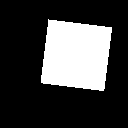
\includegraphics[width=20mm]{./input.png}};
\node [img, right= of D1] (o1) {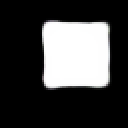
\includegraphics[width=20mm]{./output1.png}};
\node [img, right= of D2] (o2) {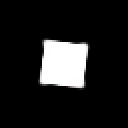
\includegraphics[width=20mm]{./output2.png}};
\node [fat arrow, right= of o1] (l1) {$\loss$};
\node [fat arrow, right= of o2] (l2) {$\loss$};
\node [img, right= of l1] (t1) {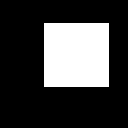
\includegraphics[width=20mm]{./target1.png}};
\node [img, right= of l2] (t2) {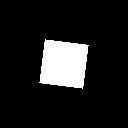
\includegraphics[width=20mm]{./target2.png}};

\end{tikzpicture}

    \caption{Schematic of the model training schedule and its functionality from left to the right by mapping the input through the encoder to $z_{\trans}$ denoted as $z_1$ and $z_{\rot}$ denoted as $z_2$ through their respective decoders leading to two different reconstructions only preserving location or rotation of the object. These then are compared with the bootstrapped $L_2$-Loss for the reconstruction loss.\\
    As can be observed in this figure the training schedule leads to the expected results for the squares dataset.} \label{model_square}
\end{figure}
The motivation of the 6D-Pose-Autoencoder is to get two latent space $z_{\rot}$ and $z_{\trans}$ from which the 6D pose comprised of rotation and translation can be read out separately.
Therefore $z_{\rot}$ encodes the orientation and should be invariant against translation while $z_{\trans}$ encodes the translation while being invariant for rotations. This is done by taking two separate Augmented Autoencoder, one for the translation and one for the rotation. They receive the same input but are trained to reconstruct differently augmented versions of the input $x_{\rot}$ and $x_{\trans}$ . The training schedule is inspired by \textbf{Hypothesis 1}.
This is achieved by applying random augmentations $f_{\text{aug}}$ comprised of a $f_{\trans}$ and $f_{\rot}$ on the input $x$. 
\begin{equation}
 \begin{aligned}
\tilde{x} = &f_{\text{aug}} (x) = (f_{\trans} \circ f_{\rot} ) (x) \\
x_{\rot} =&f_{\rot} (x) \\
x_{\trans} =&f_{\trans} (x) \\
\hat{x}_{\rot} =& (\phi_{\rot} \circ \varphi_{\rot} \circ f_{\text{aug}}) (x) \\
\hat{x}_{\trans} = &(\phi_{\trans} \circ \varphi_{\trans} \circ f_{\text{aug}}) (x)
\end{aligned}
\end{equation}
The objective function of the system thereby is:
\begin{equation}
 \begin{aligned}
\min_{\varphi_{\rot}, \phi_{\rot}}  L_{\text{rec}}(x_{\rot}, \phi_{\rot}(\varphi_{\rot}(f_{\text{aug}}(x) ))) \\
\min_{\varphi_{\trans}, \phi_{\trans}}  L_{\text{rec}}(x_{\trans}, \phi_{\trans}(\varphi_{\trans}(f_{\text{aug}}(x) ))) 
\end{aligned}
\end{equation}
For the final model $\varphi_{\rot} = \varphi_{\rot}` \circ \varphi$ and $\varphi_{\trans}= \varphi_{\trans}` \circ \varphi$ so they are encoded by the same encoder and $z_{\rot}$ and $z_{\trans}$ are just created by a split int its latent space. The complete architecture can be seen in figure \ref{model_square}.
\paragraph{Rotation} A rotation in one axis can be represented by a circle in Complex space ($\mathbb{C}$) parametrized by $\theta \in [0, 2 \pi]$ with $\exp(i \theta)$ the choice  is near to define $z_{\rot} \in \mathbb{R}^2$ and using as $L_{\text{lat}}(z) = \text{abs} (||z_{\rot}||_2^2 -1)$ which forces the encoded $z_{\rot}$ to be on the unity circle. \\ 
Rotations with three axes can be represented in a similar manner as hyper sphere in Quaternion space ($\mathbb{Q}$). So for three rotational axes we defined $z_{\rot}$ to be in $\mathbb{R}^4$ which is a generalization of $\mathbb{Q}$ with the same latent loss as stated above.\\
\paragraph{Translation} Because spatial proximity in our real world is defined by the euclidean distance in 3 dimension we chose stay as close as possible to this metric by defining the latent space for translations as follows: $z_{\trans} \in \mathbb{R}^3$. To have a dense feature space and due to the underlying metric of the real room the Euclidean norm of the latent space representations is used as regularization.
\begin{equation}
 \begin{aligned}
L_{\text{lat}}(z) = z_{\trans}^2
\end{aligned}
\end{equation}
Translations are often also easier to learn and disentangle for a neural network, traditional autoencoders on mnist for example often have translations as single latent dimensions. A fact that need to be taken into consideration with this method is that the $z$ or depth axis could also be parametrized by scale so for objects with similar shape but different scales there would also be some ambiguities.

\newpage
\subsection{Codebook}\label{Codebook}
The 6D-AE is after training able to extract the 3D orientation in $z_{\rot}$ and the translation in $z_{\trans}$. The clarity, orientation and translations of the reconstructions are a first indicator of the quality of the encodings. To extract the orientation and translation from the latent space representations we create a codebook for both rotation and translation.\\
This is done in the following way:
\begin{enumerate}
\item Render synthetic objects with known translation and rotation\\
\item Create a codebook by encoding the rendered images to $z_{\rot}\in \mathbb{R}^{O-1}$ and $z_{\trans} \in \mathbb{R}^3$ where each of those belongs to a specific rotation and translation with respect to the camera
\end{enumerate}
The next step is to utilize the K-Nearest-Neighbour algorithm separately on the two latent space representations of the test images with unknown labels compared to the codebook with known labels.\\
The Distance metric used for the rotations $z_{\rot}$ is the cosine similarity. This is done because we initially made the assumption that our representations lie in a hyper sphere with unit distance from the origin.
\begin{equation}
\cos_i = \dfrac{z_i \cdot z_{\text{test}}}{ \vert\vert  z_i \vert \vert \cdot \vert \vert z_{\text{test}} \vert \vert }
\end{equation}
For the translation the euclidean distance was chosen as distance metric to determine the next nearest neighbours and instead of the naive kNN algorithm a with softmax weighted algorithm was used to compute the location of the object $\vec{y}$. 
\begin{equation}
\vec{y}(z_{\trans}) = \dfrac{\sum_j  \vec{y}_j  \cdot  \exp(- L_2(z_{\trans},z_{\trans , j})) }{\sum_j \exp(- L_2(z_{\trans},z_{\trans , j}))}
\end{equation}



\newpage
\section{Evalutation}\label{Evaluation}
In the following section we present our results as well as the methods used to investigate the behaviour of the 6D-AE and to verify the assumptions made in the chapter methods \ref{Methods}.
\subsection{2D Square in 3D Space}\label{Square}
In this experiment we focused on reproducing the qualitative results of the Augmented Autoencoder which can be seen in figure \ref{SQUARE_Martin} and disentangling the latent space representation of the translation and rotation with the training scheme represented in the chapter \ref{6D Pose Autoencoder}. The resulting reconstructions allow conclusion on the orientation of the square and only contain either translation or rotation. They can be seen in figure \ref{square_images} in the appendix.\\
$z_{\rot}$ was defined to be in in $\mathbb{R}^2$ representing $\mathbb{C}$ as described in chapter \ref{Methods} due to the single rotation axis of the object. Due to the two perpendicular axes of symmetry the square posses we anticipated to see a shifted and cosine function with the frequency $f = 2/ \pi$, because the square appears exactly the same after a rotation of $\dfrac{\pi}{2}i$. \\
The second part was to show that the translation could be extracted from the latent space representation $z_{\trans}$ and that different rotations have neglegible effect on it. The resulting plot for the correlation between $z_{\rot}$ and the rotation $\varphi$ as well as $z_{\trans}$ and the translation can be seen in figure \ref{Square_corr_rot} and \ref{Square_corr_trans}. 
The plot for $\theta$ shows a periodic behaviour with the correct correct frequency but not the predicted cosine and sine.
\begin{figure}[!ht]
\centering
\begin{subfigure}{0.49\textwidth}
	\centering
	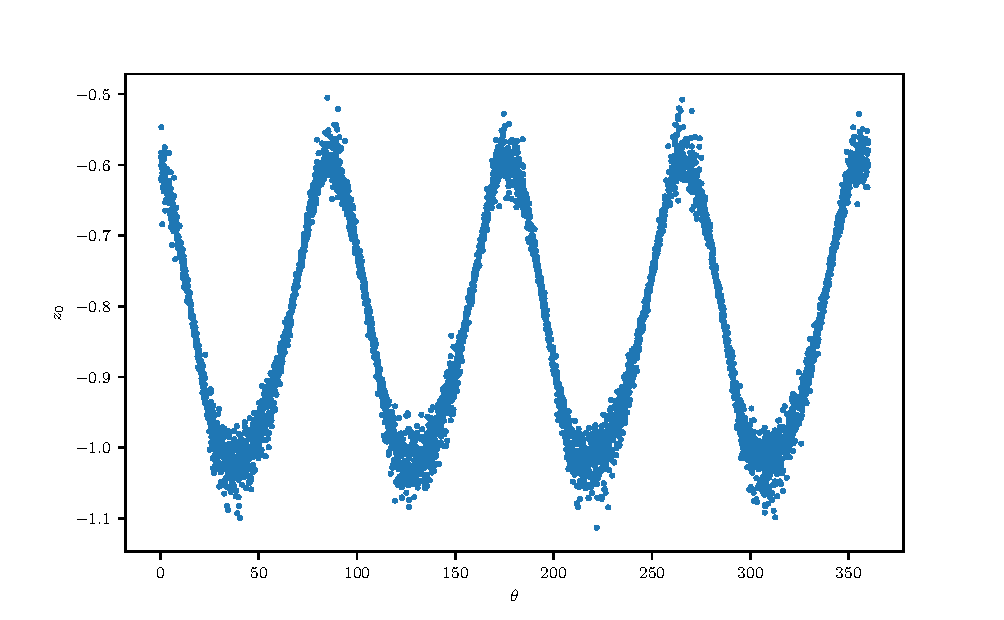
\includegraphics[width=\textwidth] {square_theta_z0.pdf}
	\caption{}
	\label{fig_zo}
\end{subfigure}
\begin{subfigure}{0.49\textwidth}
	\centering	
	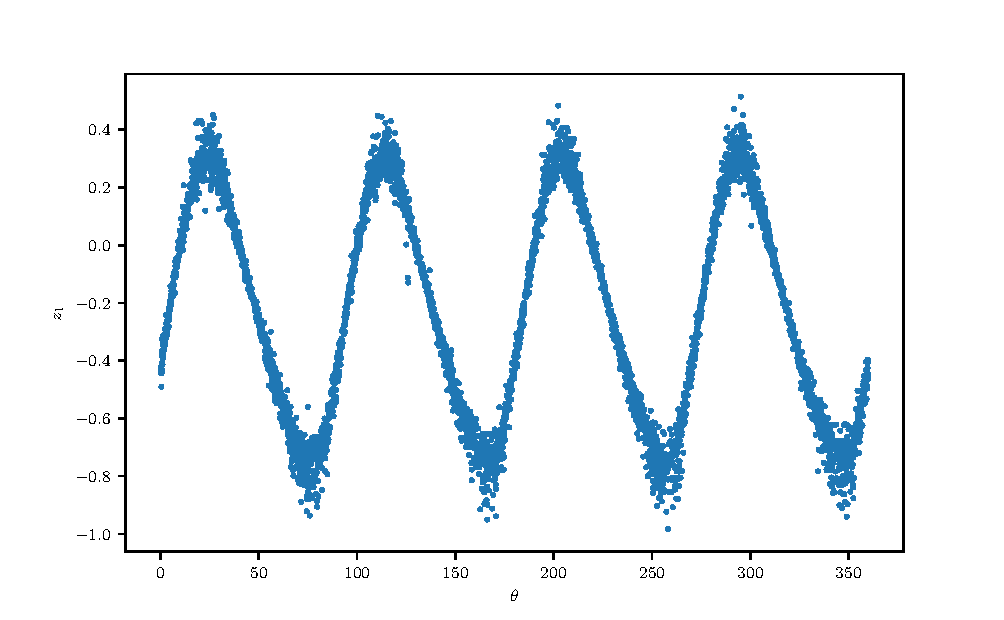
\includegraphics[width=\textwidth]{square_theta_z1.pdf}
	\caption{}
	\label{fig_z1}
\end{subfigure}
\caption{Correlation plots of the rotation $\theta$ and the dimensions of $z_{\rot}$.\\
The values show a period of $\pi/2$ representing the symmetries of the square even though they do not show the anticipated behaviour of being cosine and sine.} \label{Square_corr_rot}
\end{figure}
In table \ref{square_results} it can be observed that the rotations and translations behave differently with the parameter $k$ of the codebook prediction. The prediction of the translation gets worse with increasing $k$ even though due to the weighted $kNN$ prediction. Whereas the predicted orientation of $\theta$ gets better with increasing $k$ but the best metric for the $kNN$ prediction is not the cosine as supposed but the euclidean similarity metric.

\begin{table}
    \begin{adjustbox}{width=\textwidth}
        \begin{tabular}[width = \textwidth]{lccccccccc} 
    Metric & \multicolumn{6}{c}{RMSE} & mean vsd & recall & mean cosine \\
           &&&&&&&&& similarity \\
    \hline
    Parameter & $\theta$ & $\phi$ & $\gamma$ & $x_{\text{ax}}$  &
    $y_{\text{ax}}$ & $z_{\text{ax}}$ &       &      & angles\\
\hline
Square        & 0.73     &        &          & 0.04             & 0.04            & 0.20            & 0.06  & 1.00 & 1.00 \\
CUBE 4        & 14.10    & 12.80  &          & 0.06             & 0.06
              & 0.19     & 0.12   & 0.99     & 0.96            \\
CUBE 64       & 7.27    & 6.15  &          & 0.05             & 0.05
              & 0.16     & 0.10   & 0.99     & 0.97            \\
CAT 4         & 107.07   & 77.48  & 105.04   & 0.12             & 0.13
              & 0.34     & 0.54 & 0.03 & 0.51    \\
CAT 64        & 112.51   & 75.27  & 111.50   & 0.13             & 0.13
              & 0.31     & 0.51 & 0.08 & 0.53    \\
\end{tabular}
\end{adjustbox}
\caption{Evaluation metrics for the different datasets}
\label{square_results}
\end{table}

Additionally we interpolated in the $z_{\trans}$ and $z_{\rot}$ space. There it verifies that our assumptions about the unity circle were not correct because it did not show the anticipated behaviour for the rotations which can be observed in figure \ref{square_ipol}.
The interpolations in $z_{\trans}$ can be seen in figure \ref{square_ipol} and behave as anticipated by representing the translations where the scaling or depth translation is entangled with all 3 dimensions of $z_{\trans}$. A possible explanation for this is that the learned representation is a coordinate system with a linear transformation of the real coordinates.\\  
\begin{figure}[!ht]
\centering
\begin{subfigure}{0.49\textwidth}
	\centering
	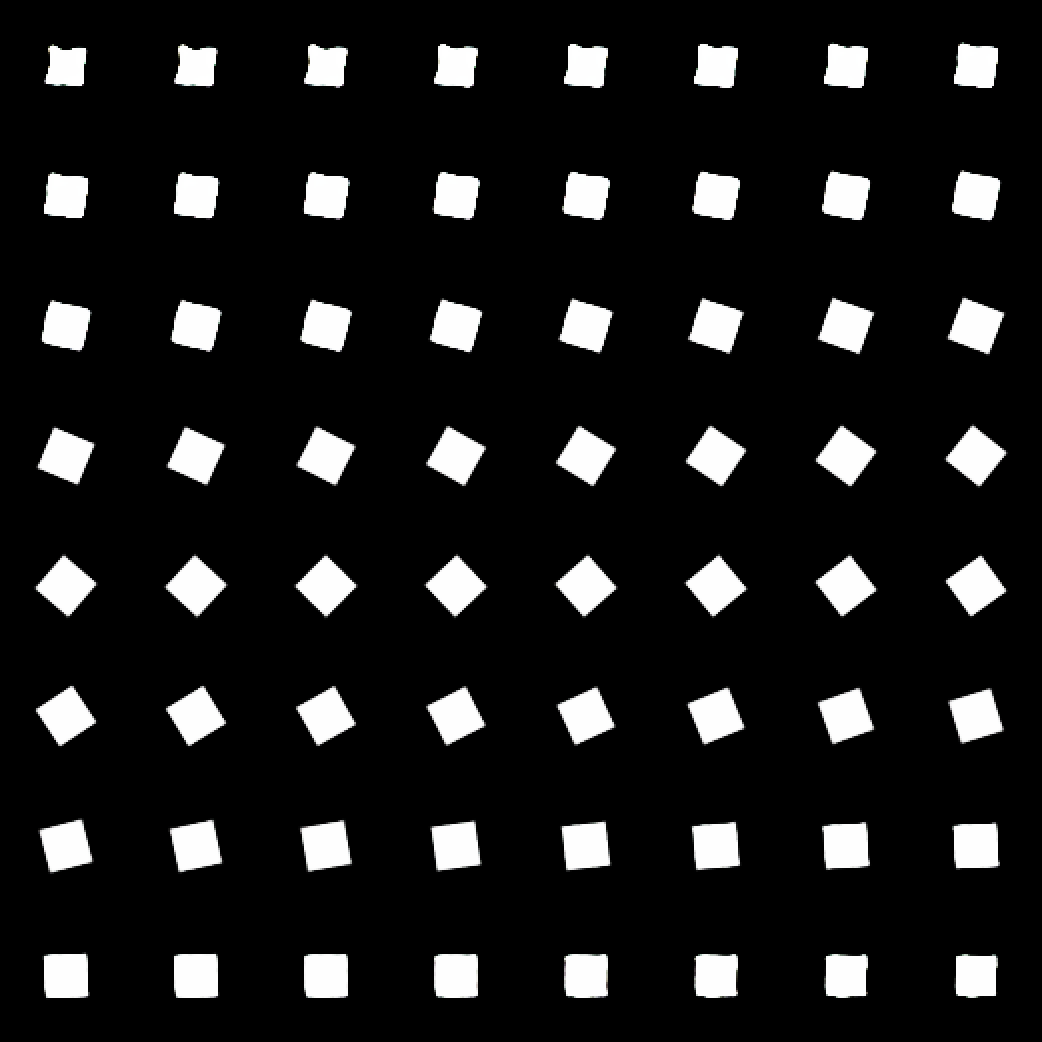
\includegraphics[width=\textwidth] {square_interpolation_theta.png}
	\caption{}
	\label{fig1:subim1}
\end{subfigure}
\begin{subfigure}{0.49\textwidth}
	\centering	
	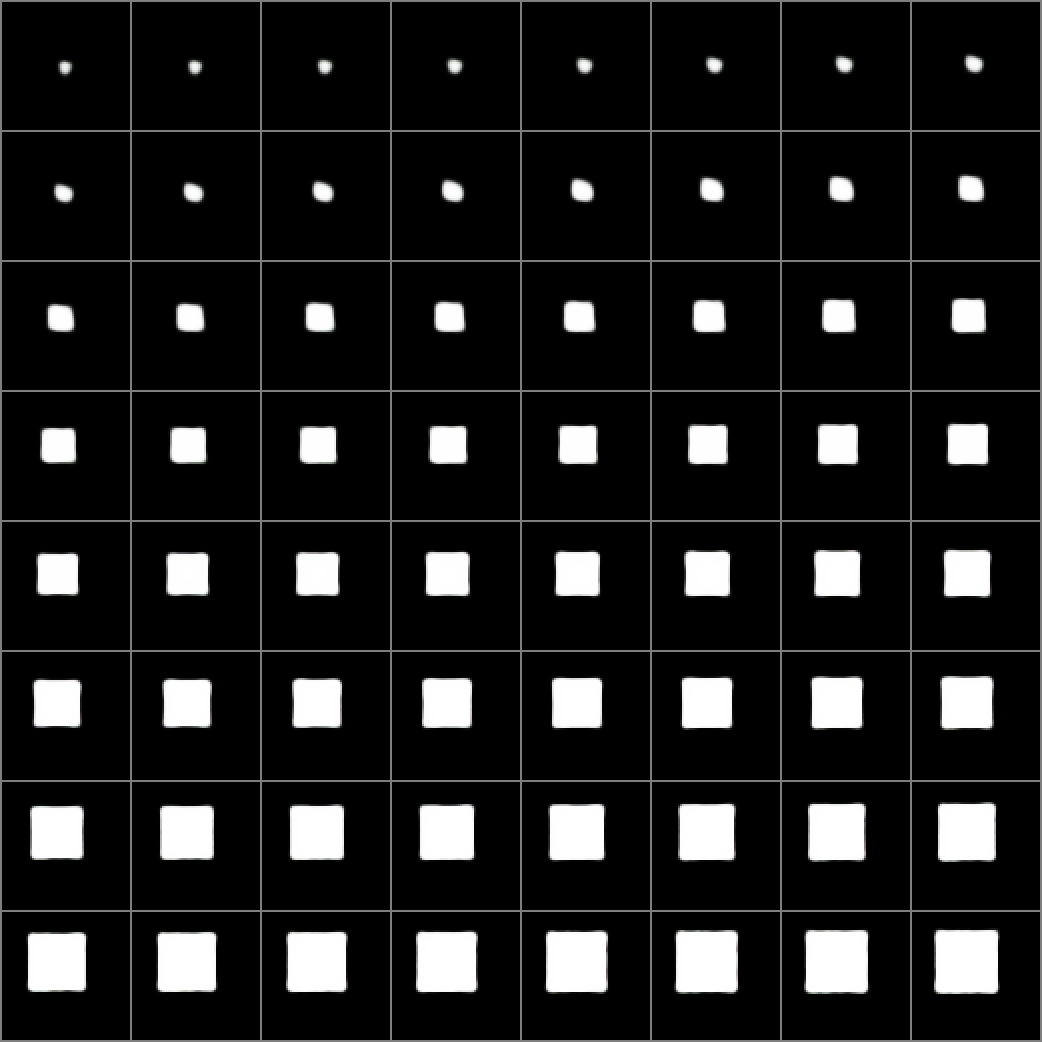
\includegraphics[width=\textwidth]{square_interpolation_x.png}
	\caption{}
	\label{fig1:subim2}
\end{subfigure}
\begin{subfigure}{0.49\textwidth}
	\centering	
	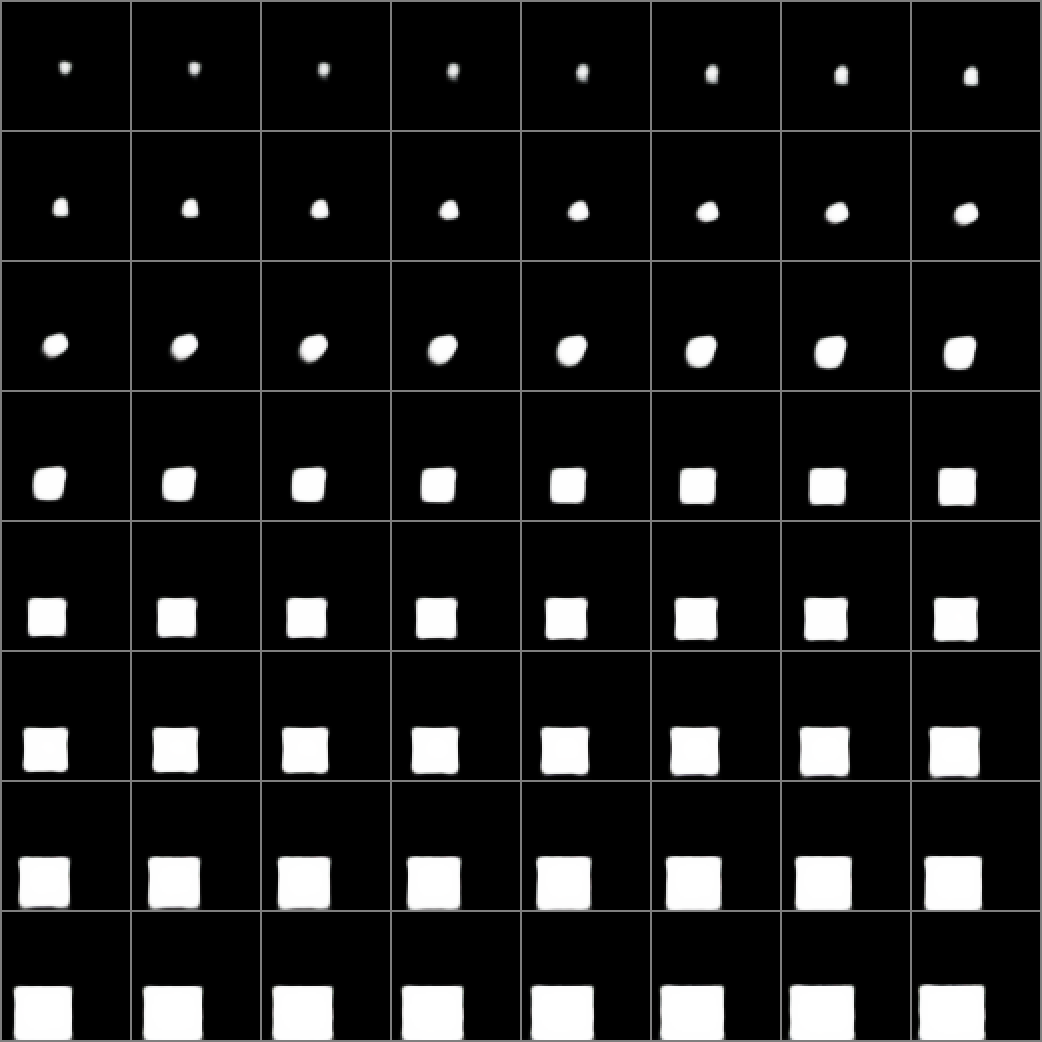
\includegraphics[width=\textwidth ] {square_interpolation_y.png}
	\caption{}
	\label{fig1:subim3}
\end{subfigure}
\begin{subfigure}{0.49\textwidth}
	\centering	
	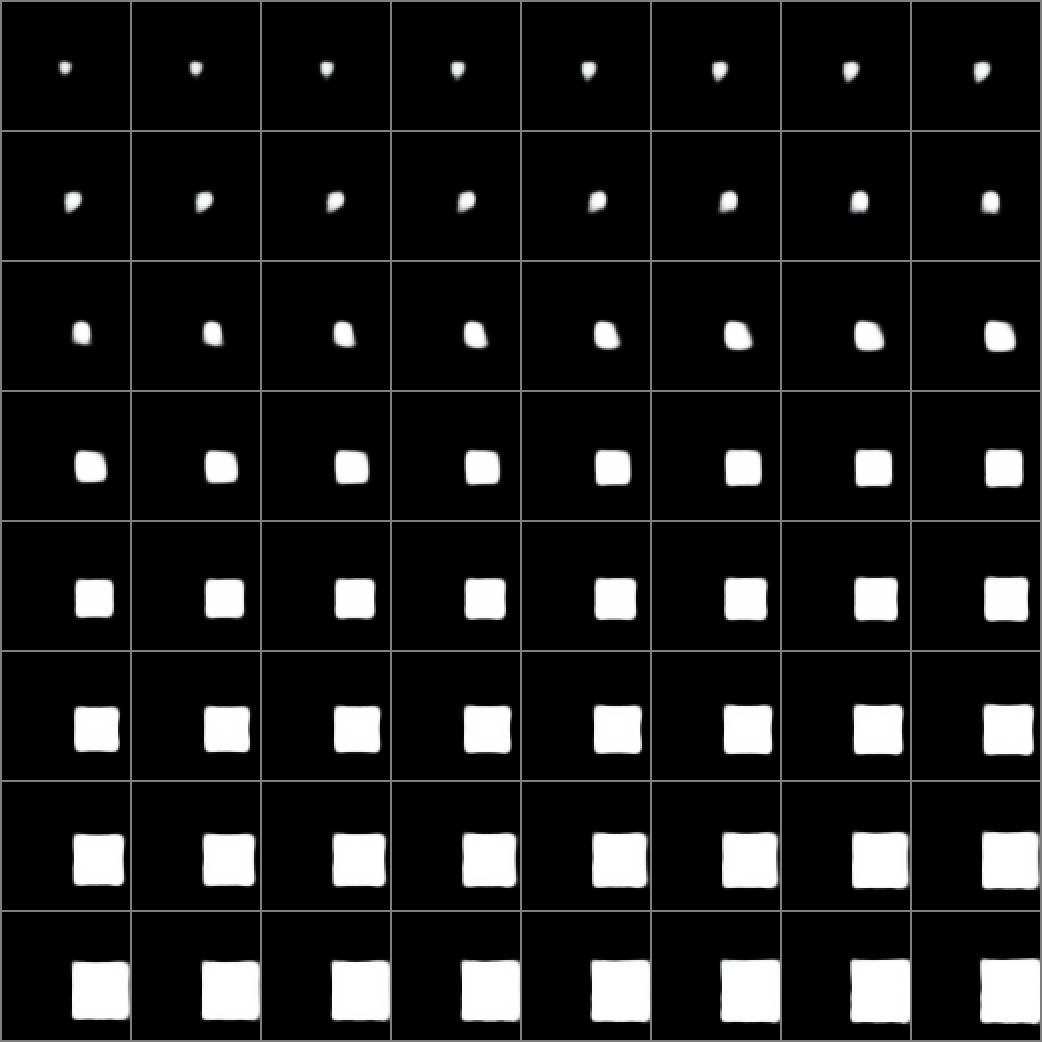
\includegraphics[width=\textwidth] {square_interpolation_z.png}
	\caption{}
	\label{fig1:subim4}
\end{subfigure}
\caption{Interpolations: (a) in $\alpha \in (\pi /2, 3/2 \pi)$ with $z_{\rot}= (cos(\alpha), sin(\alpha))^T$\\
(b), (c) and (d) linear interpolations from 0 to 2 in $z_{\trans_{1/2/3}}$ with other dimensions set to 0.\\
All 3 dimensions seem to represent the translation in the $z$ axis and a different mixture of $x$ and $y$ axis which appears to be linearly separable according to (b), (c) and (d).} \label{square_ipol}
\end{figure}
\newpage
\subsection{3D Cube}\label{Cube}
In this experiment we wanted to expand our predictions to a more complex case by taking the next complex object from the 2D square in 3D, namely the 3D cube. the 3D cube gets rotated in 2 axes due to trivial reasons of symmetry which leads to the conclusion that the rotations should be able to be represented by a hyper-sphere in 4 dimensions. So $z_{\rot}$ was chosen to be element of $\mathbb{R}^4$. The correlations between $z_{\rot}$ can be seen in figure \ref{cube_corr_rot}. \\
The correlations for the translation, which can be seen in figure \ref{cube_corr_trans}, also lead to the conclusion of $z_{\trans}$ being a linear transformation of the translations. 
\begin{figure}[!ht]
\centering
\begin{subfigure}{0.49\textwidth}
	\centering
	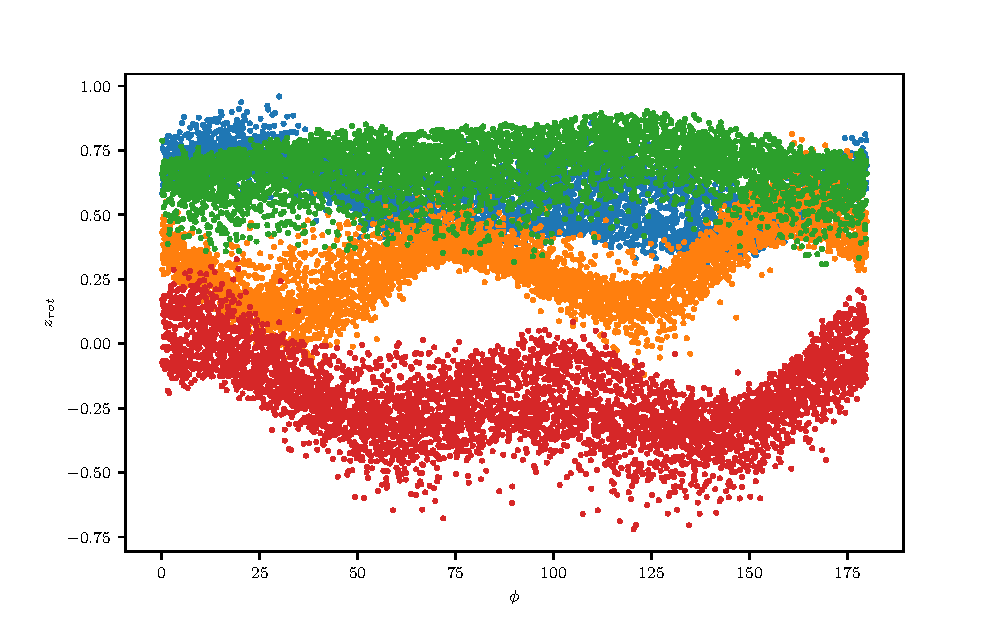
\includegraphics[width=\textwidth] {cube_rot_phi_z_all.pdf}
	\caption{}
	\label{fig_rotph_all}
\end{subfigure}
\begin{subfigure}{0.49\textwidth}
	\centering	
	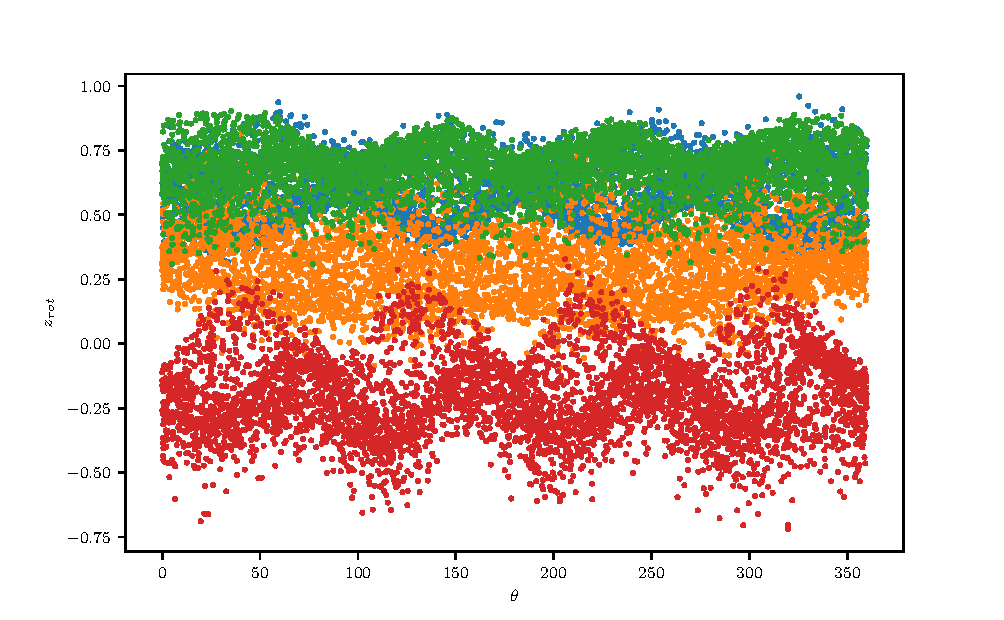
\includegraphics[width=\textwidth]{cube_rot_theta_z_all.pdf}
	\caption{}
	\label{fig_rotth_all}
\end{subfigure}
\caption{Correlation plots of the rotation $\theta$ as well as $\phi$ and the dimensions of $z_{\rot}$.\\
The different dimensions are differently colored and show clear periodic behaviour.} \label{cube_corr_rot}
\end{figure}


\newpage
\subsection{Line Mod: Cat}
The final experiment was conducted on the Cat of the Line Mod dataset which is created by Stefan Hinterstoisser \cite{LINEMOD}.
The cat is a much more complex object than the cube with no symmetries and more contours. Also we added the third rotation leading to now complete Euler angles for the rotations. The training used is identically to schedule for cubes and squares. \\
The lack of any symmetries would be a powerful way to prove that the 3 Euler rotations can be represented by the unity sphere in $\mathbb{R}^4$, a generalization of the quaternions $\mathbb{Q}$.\\
Because the reconstructions of this the AAE with $z_{\rot}$ being 4 dimensional were not satisfying which is why decided to also train a model with $z_{\rot}$ being 64 dimensional. The reconstructions of both models can be seen in figure \ref{cat_images} where the reconstructions of the model with 4 latent rotational dimensions has washed out reconstruction with ambiguous rotations, where head and body cannot clearly be separated. \\
Also we could not find any correlations in the rotational latent space to any euler angle for Model 1. Due to the big latent space we did not even attempt to find correlations by hand for Model 2. Our only way to verify the quality of the latent space thereby is the prediction of the correct pose via the codebook for Model 2 and also Model 1. \\




 Both reconstructions can be seen in figure \ref{cat_images}. The vsd errors for both of these models where: XXXXXXXXXX

\begin{figure}[!ht]
\centering
\begin{subfigure}{\textwidth}
	\centering
	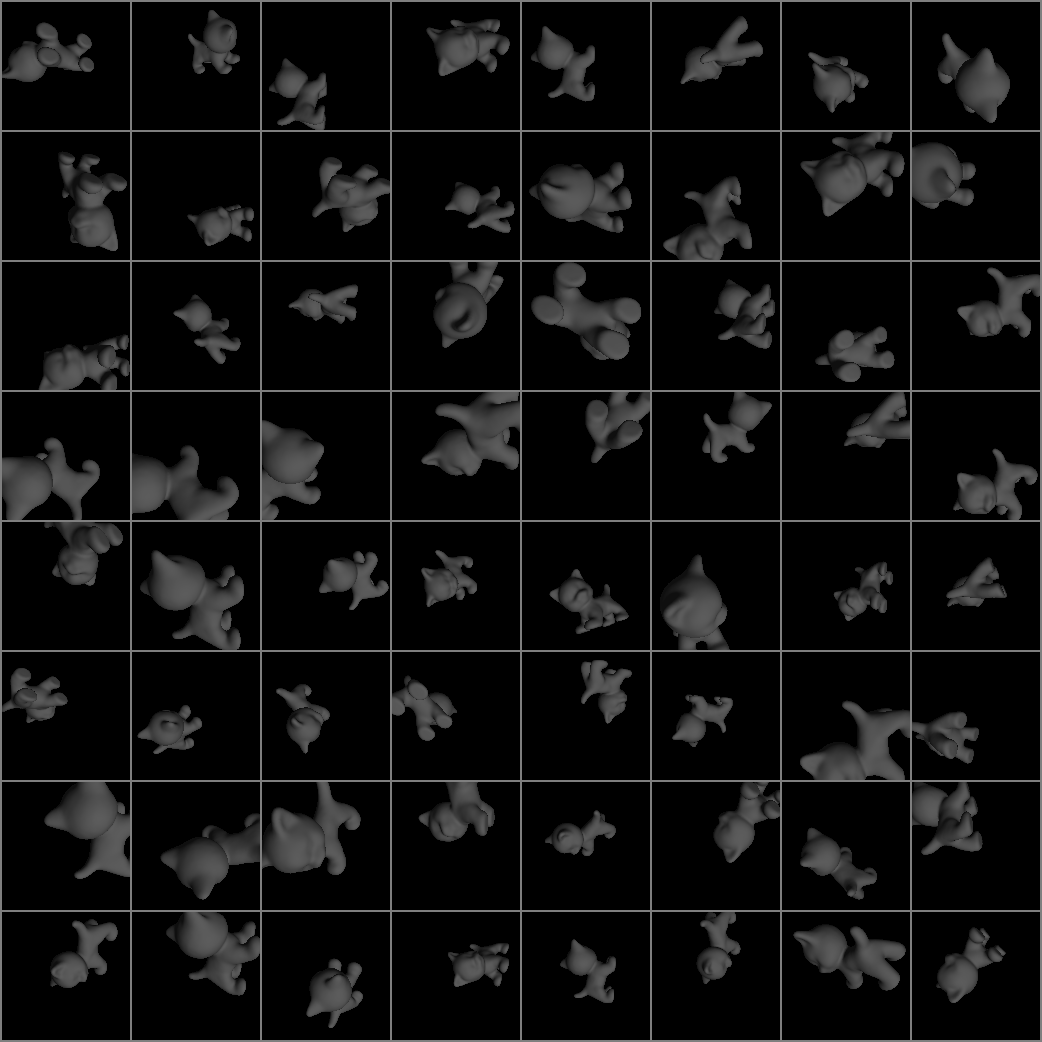
\includegraphics[width=0.49\textwidth] {cat_input.png}
	\caption{Input}
	\label{cat_in}
\end{subfigure}
\begin{subfigure}{0.3\textwidth}
	\centering
	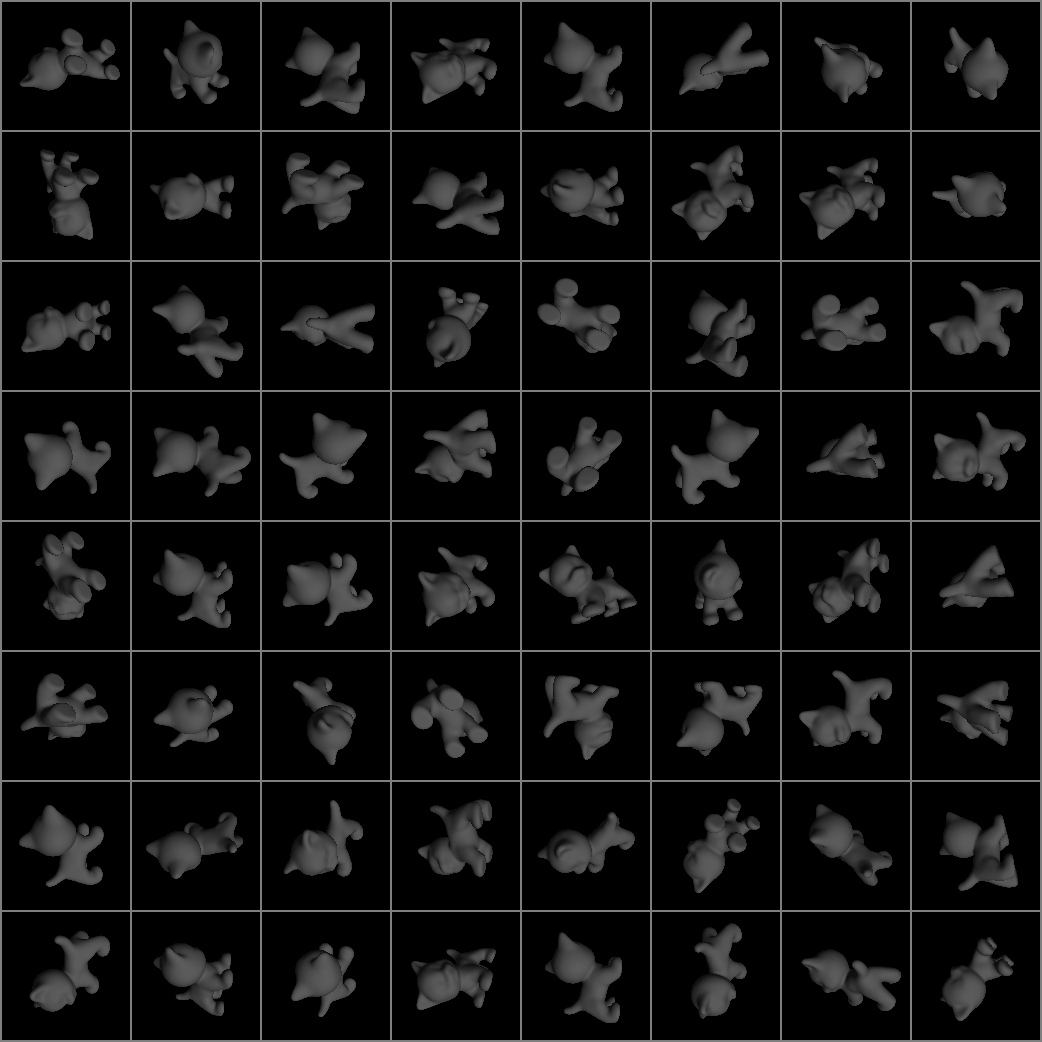
\includegraphics[width=\textwidth] {cat_target0.png}
	\caption{Rotation target}
	\label{cat_r}
\end{subfigure}
\begin{subfigure}{0.3\textwidth}
	\centering
	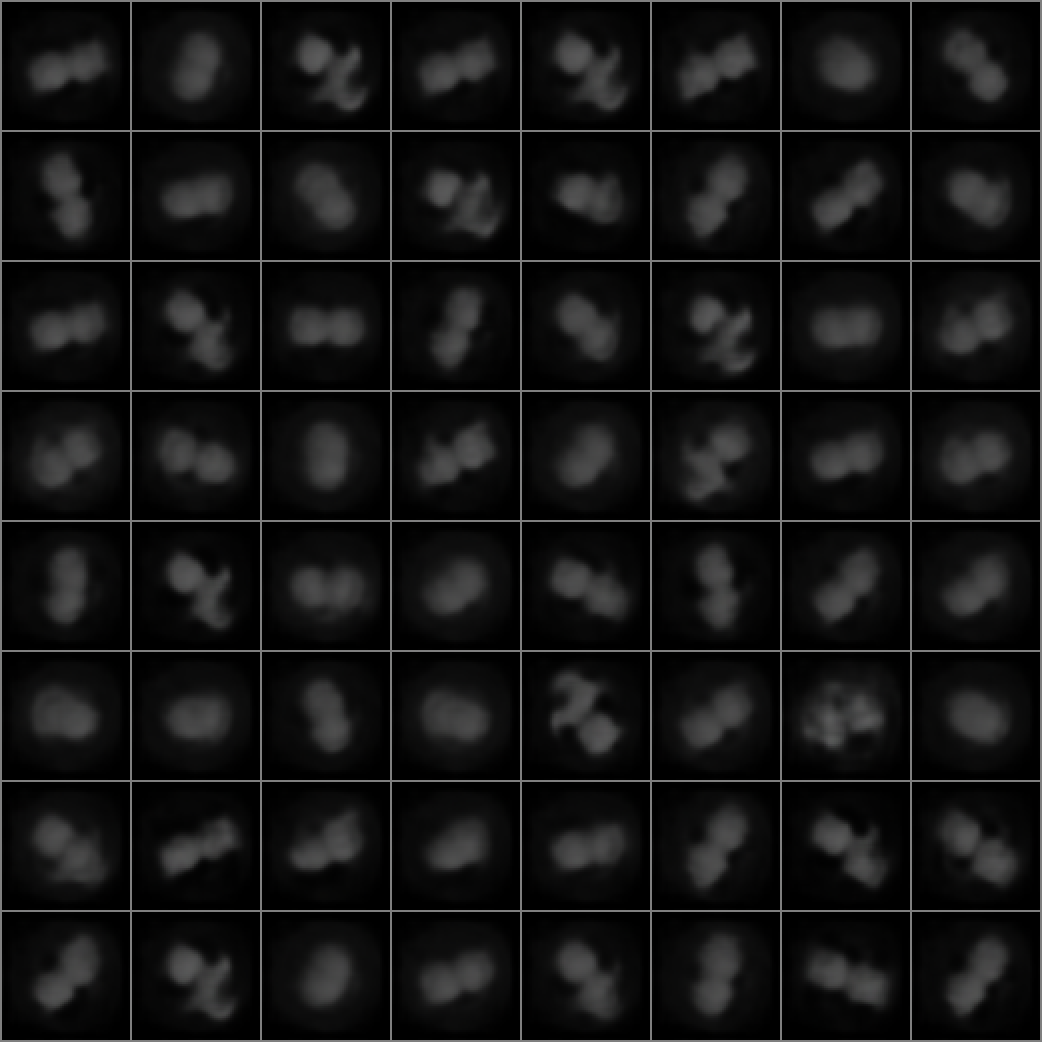
\includegraphics[width=\textwidth] {cat_4_output0.png}
	\caption{Rotation Model 1}
	\label{cat_rrec}
\end{subfigure}
\begin{subfigure}{0.3\textwidth}
	\centering
	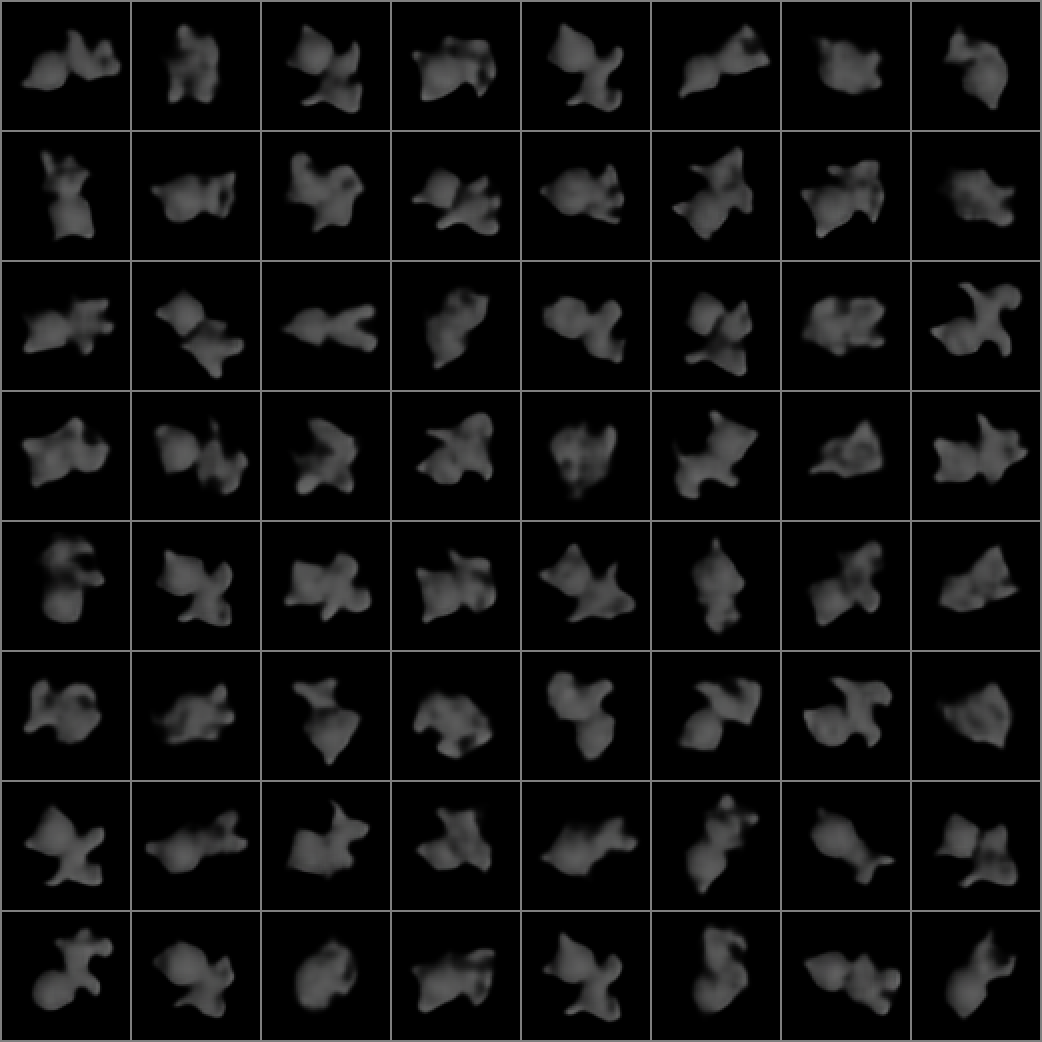
\includegraphics[width=\textwidth] {cat_64_output0.png}
	\caption{Rotation Model 2}
	\label{cat_rrec2}
\end{subfigure}

\begin{subfigure}{0.3\textwidth}
	\centering	
	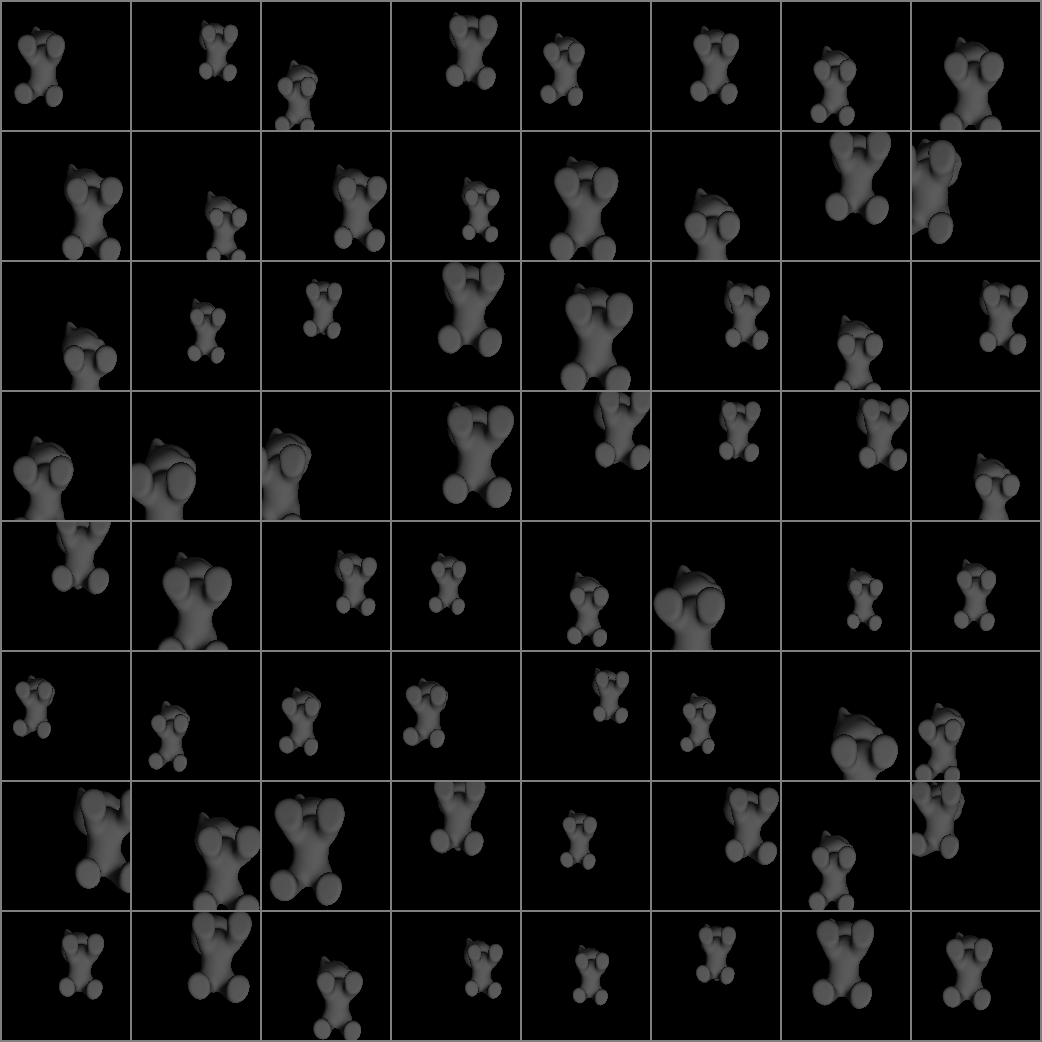
\includegraphics[width=\textwidth]{cat_target1.png}
	\caption{Translation target}
	\label{cat_t}
\end{subfigure}
\begin{subfigure}{0.3\textwidth}
	\centering	
	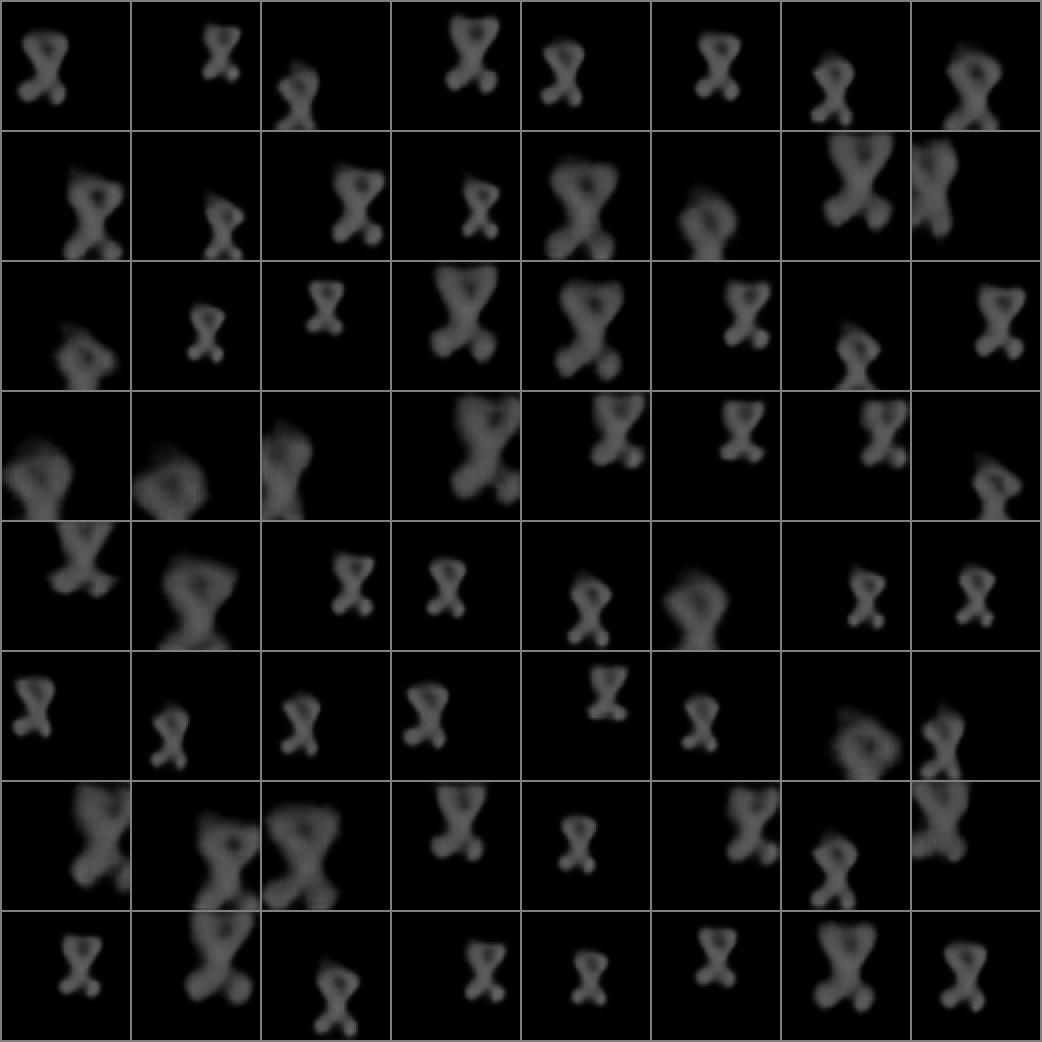
\includegraphics[width=\textwidth]{cat_4_output1.png}
	\caption{Translation Model 1}
	\label{cat_trec}
\end{subfigure}
\begin{subfigure}{0.3\textwidth}
	\centering	
	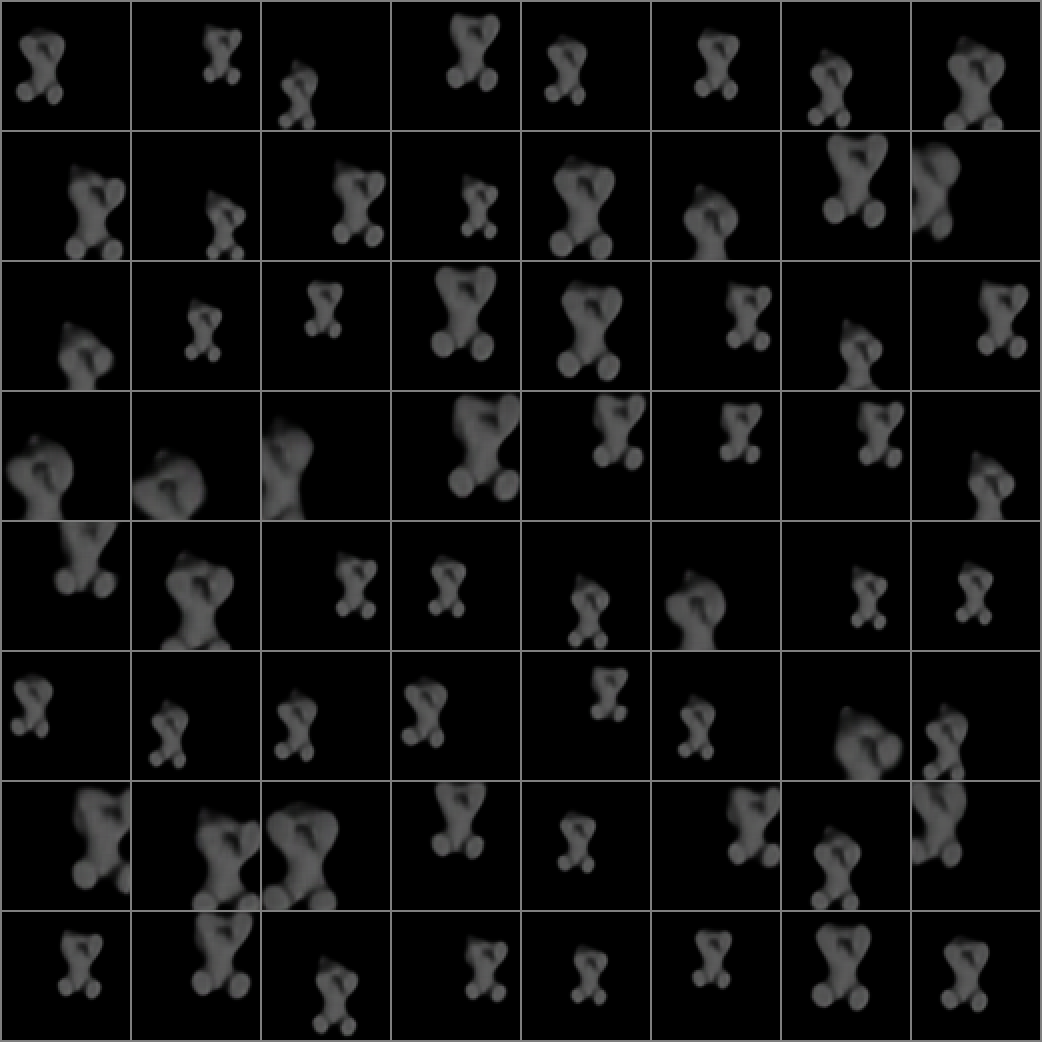
\includegraphics[width=\textwidth]{cat_64_output1.png}
	\caption{Translation Model 2}
	\label{cat_trec1}
\end{subfigure}
\caption{Comparision between reconstructions and targets of the two AAEs. 
Dimensions of $z_{\rot}$: 4 for Model 1 and 64 for Model 2.\\
The reconstructions of Model 2 show much more detail and are less ambiguous regarding to the reconstructed rotation than the reconstructions of Model 1.} \label{cat_images}
\end{figure}

\newpage
\section{Conclusion}


The general concept of this work namely the split in rotational latent space $z_{\rot}$ and translational latent space $z_{\trans}$ of the augmented autoencoder was shown to work  extremely well by restricting the size of the latent space in experiments A TO B.\\
We were able to extract the 3D orientation as well as the 3D rotation with regard to the camera of the object with the codebook.\\
\\
The connection between $N$-dimensional rotations and the $N-1$-dimensional unity sphere was shown to be appropriate and used to minimize the size of the latent space in the experiment SQUARE and CAT\\
\\
In general this model thereby allows a more accurate estimation of the 3D translation than the model presented by martin sundermeier et. al. .
It is also easily able to detect on which object the network is basing its prediction of the codebook by checking the translation reconstruction in case of misspredictions or multiple objects of the same class.\\

 
\newpage
\section{Sources}\label{Sources}
\printbibliography

\newpage
\section{Appendix}
\begin{figure}
\center
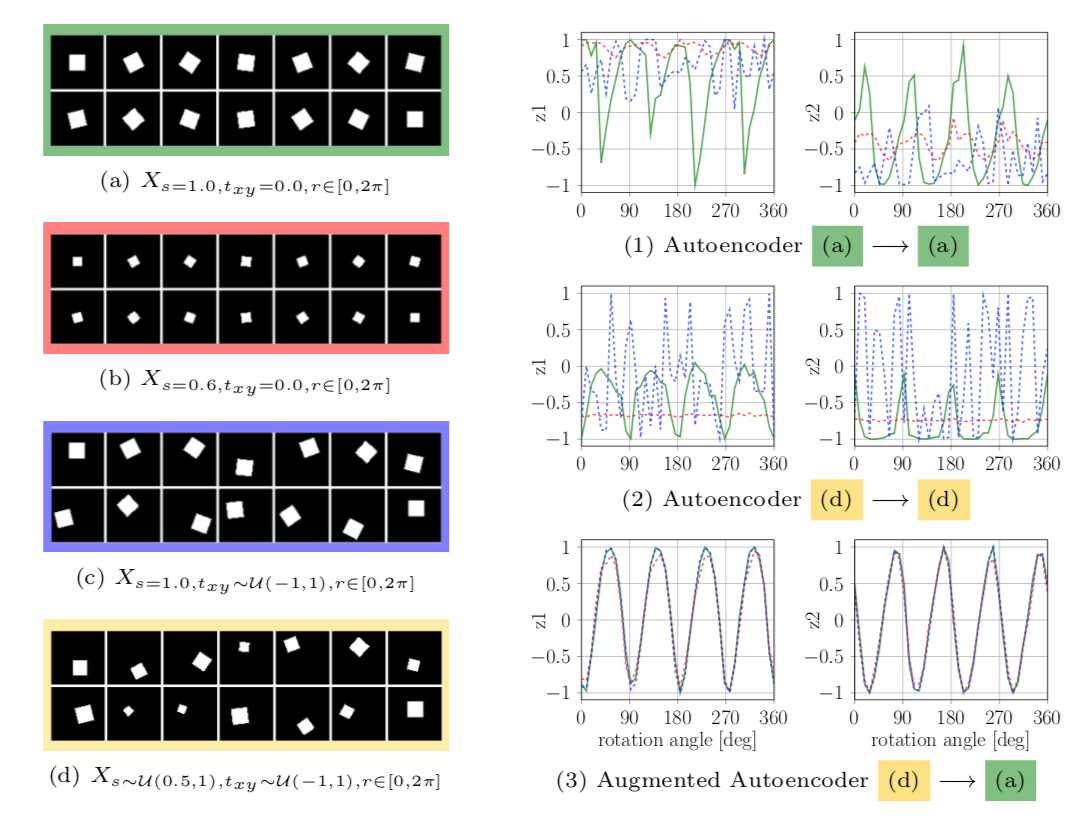
\includegraphics[width = \linewidth]{MARTIN_Squares.png}
\caption{Results presented by Martin et al. in \cite{3D_Orientation_Learning} to compare with our results for square in fig \ref{square_ipol}
Left: squares from the distributions (a,b,c and d) with different translations in x,y and z axis used for training and testing\\
Right: Normalized latent dimensions $z_{\rot_1}$ and $z_{\rot_2}$ for the rotations of the distributions from (a-d). (1-2) are from normal AEs whereas (3) is from the AAE.}\label{SQUARE_Martin}
\end{figure}


\begin{figure}[!ht]
\centering
\begin{subfigure}{\textwidth}
	\centering
	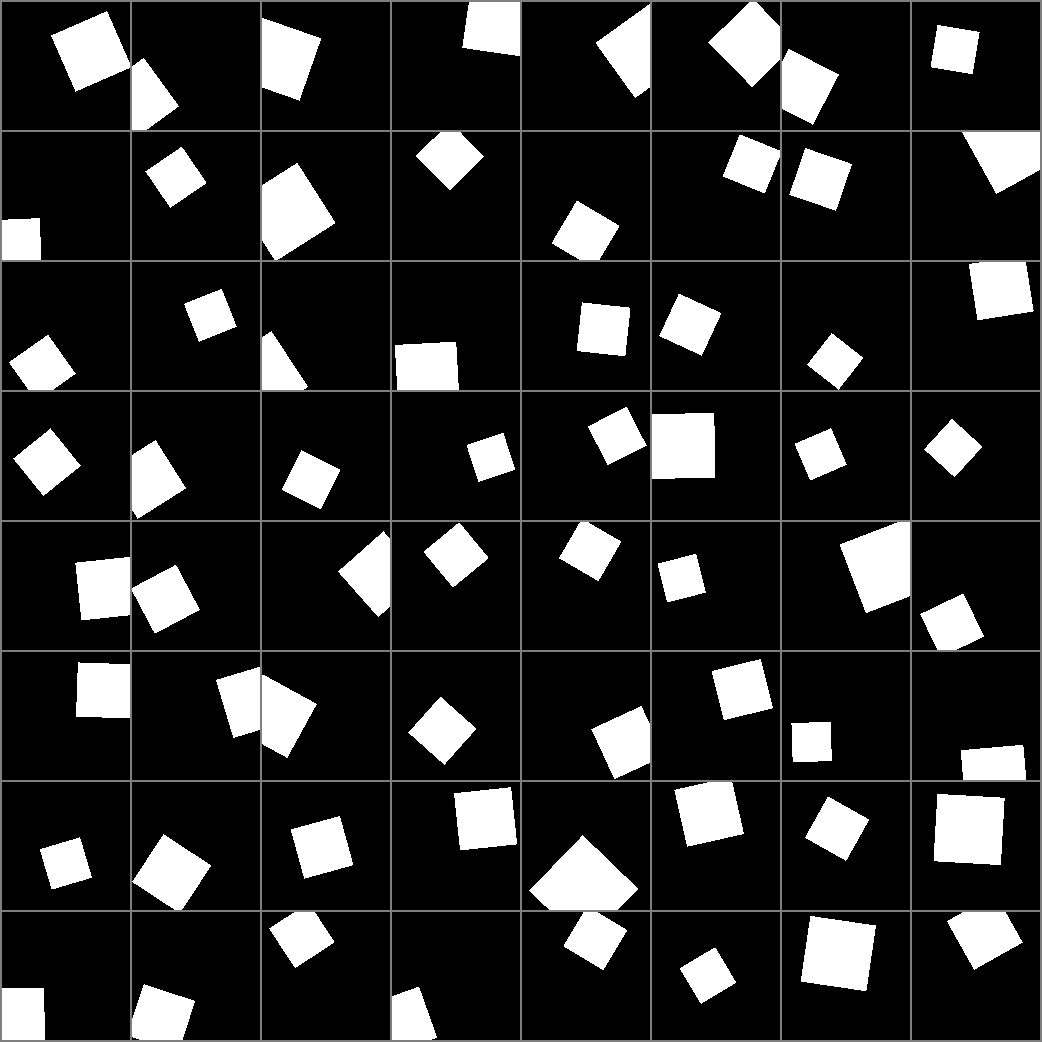
\includegraphics[width=0.49\textwidth] {square_input.png}
	\caption{Input}
	\label{sq_in}
\end{subfigure}
\begin{subfigure}{0.49\textwidth}
	\centering
	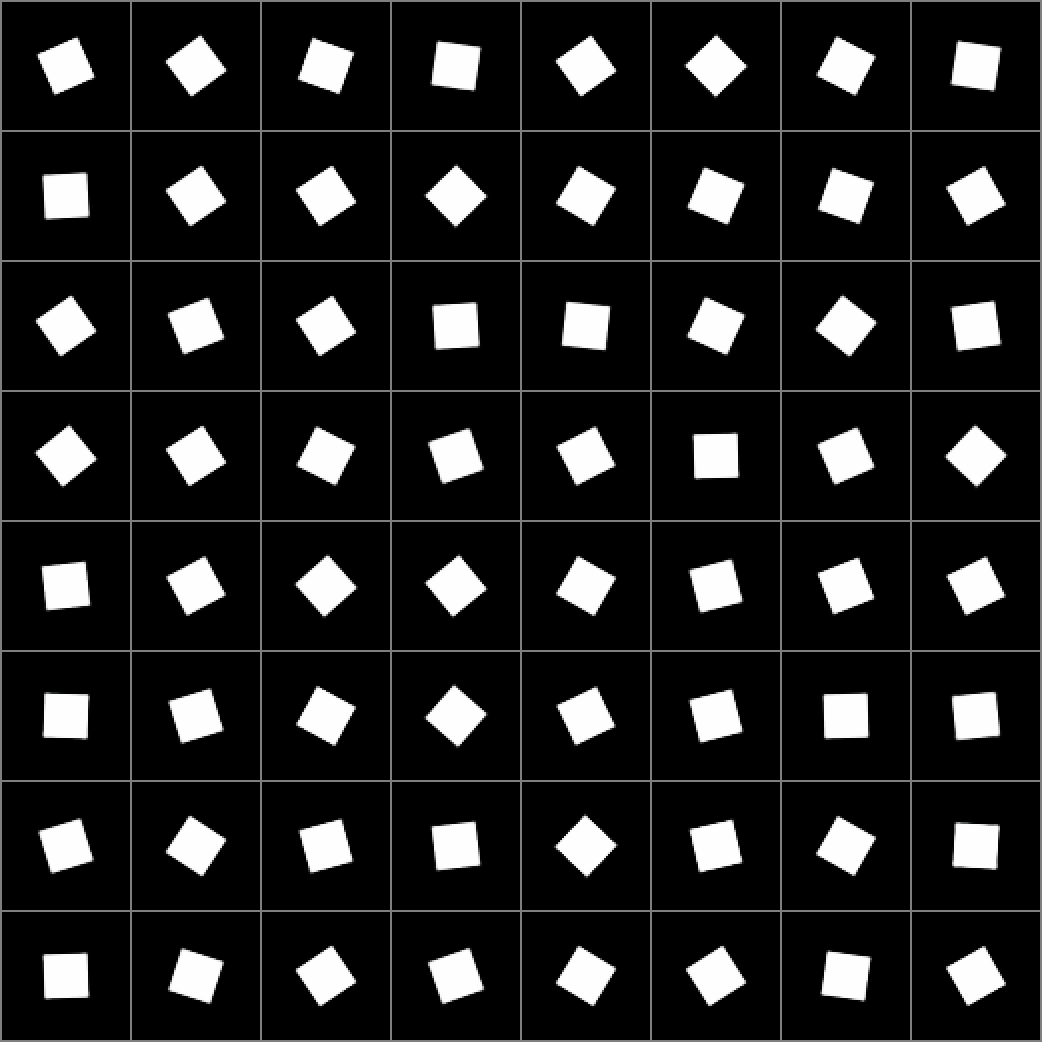
\includegraphics[width=\textwidth] {square_output0.png}
	\caption{Translation reconstr.}
	\label{sq_trec}
\end{subfigure}
\begin{subfigure}{0.49\textwidth}
	\centering	
	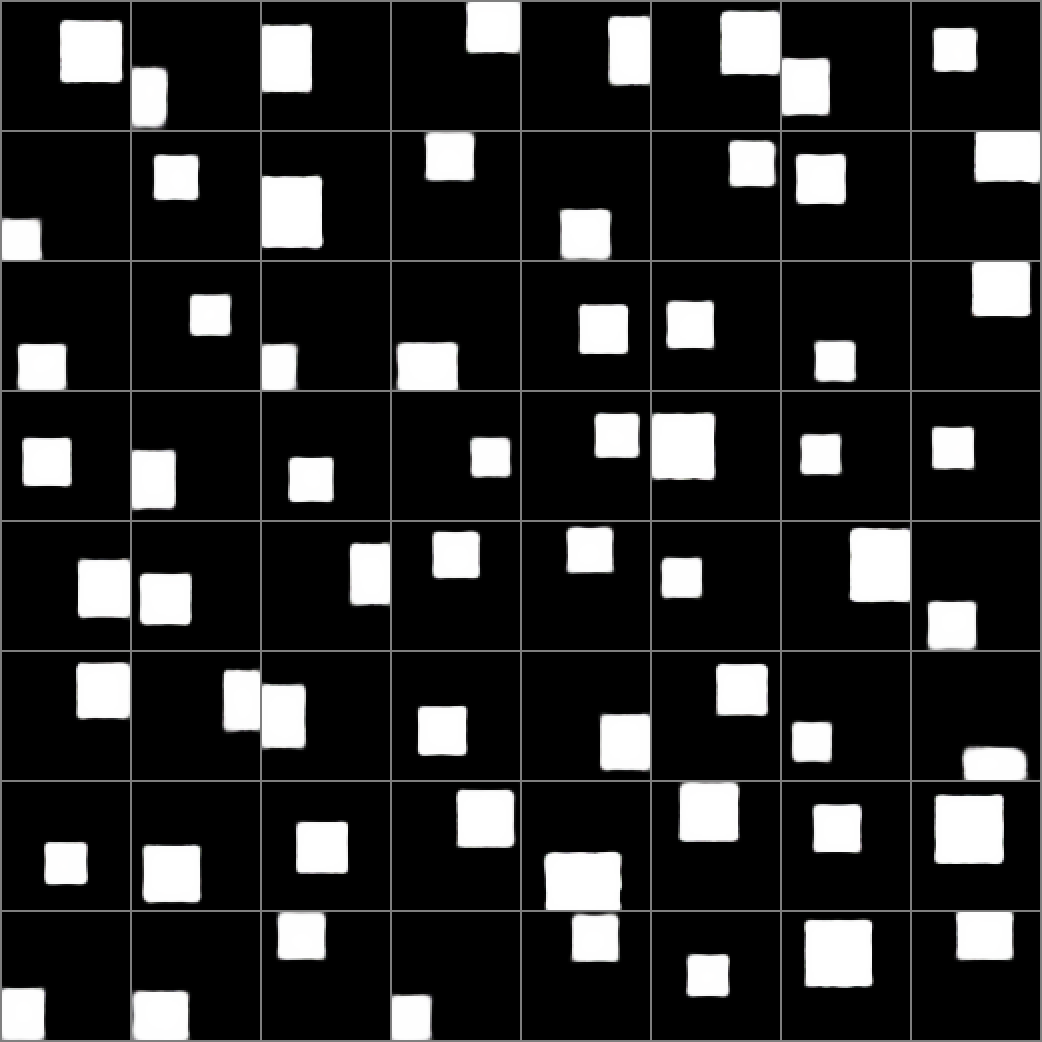
\includegraphics[width=\textwidth]{square_output1.png}
	\caption{Rotation reconstr.}
	\label{sq_rrec}
\end{subfigure}
\begin{subfigure}{0.49\textwidth}
	\centering
	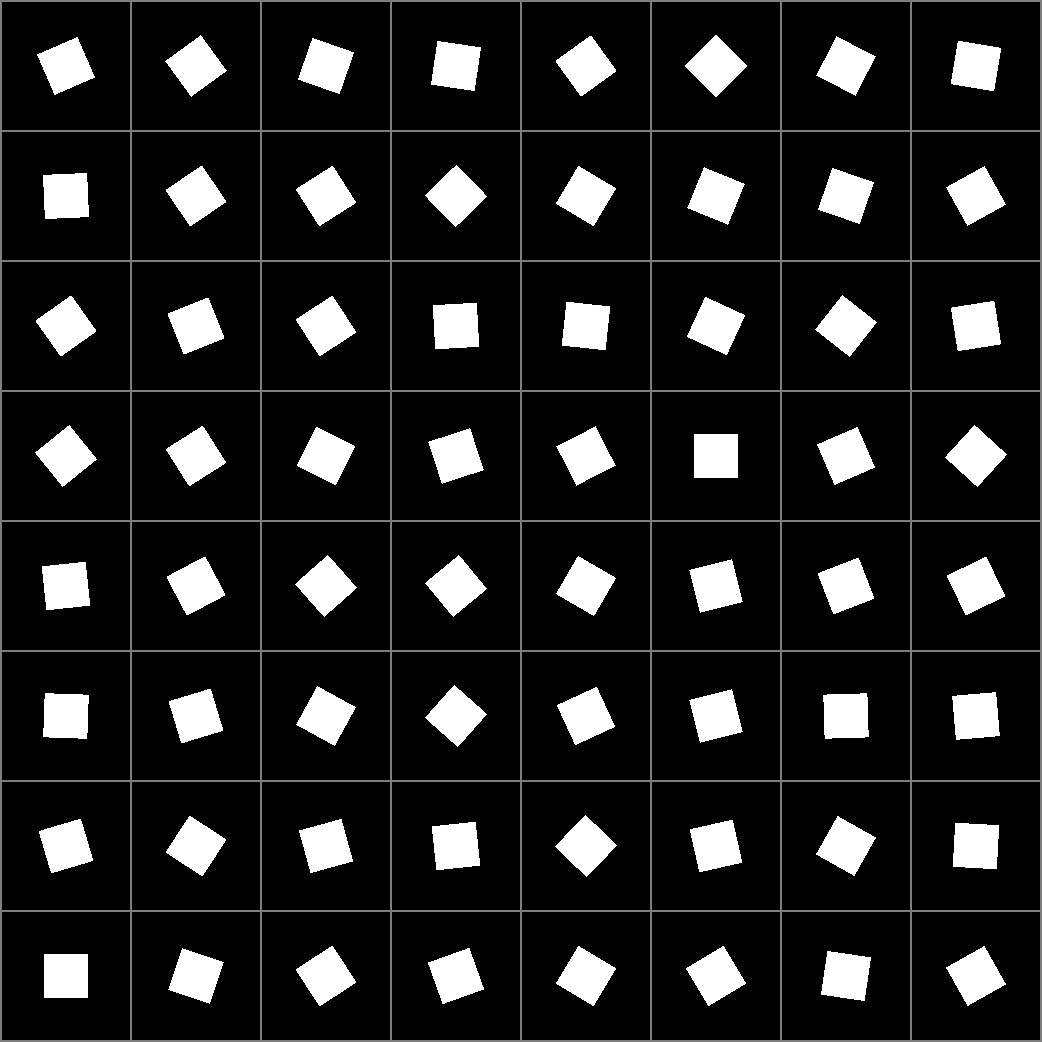
\includegraphics[width=\textwidth] {square_target0.png}
	\caption{Translation target}
	\label{sq_tt}
\end{subfigure}
\begin{subfigure}{0.49\textwidth}
	\centering	
	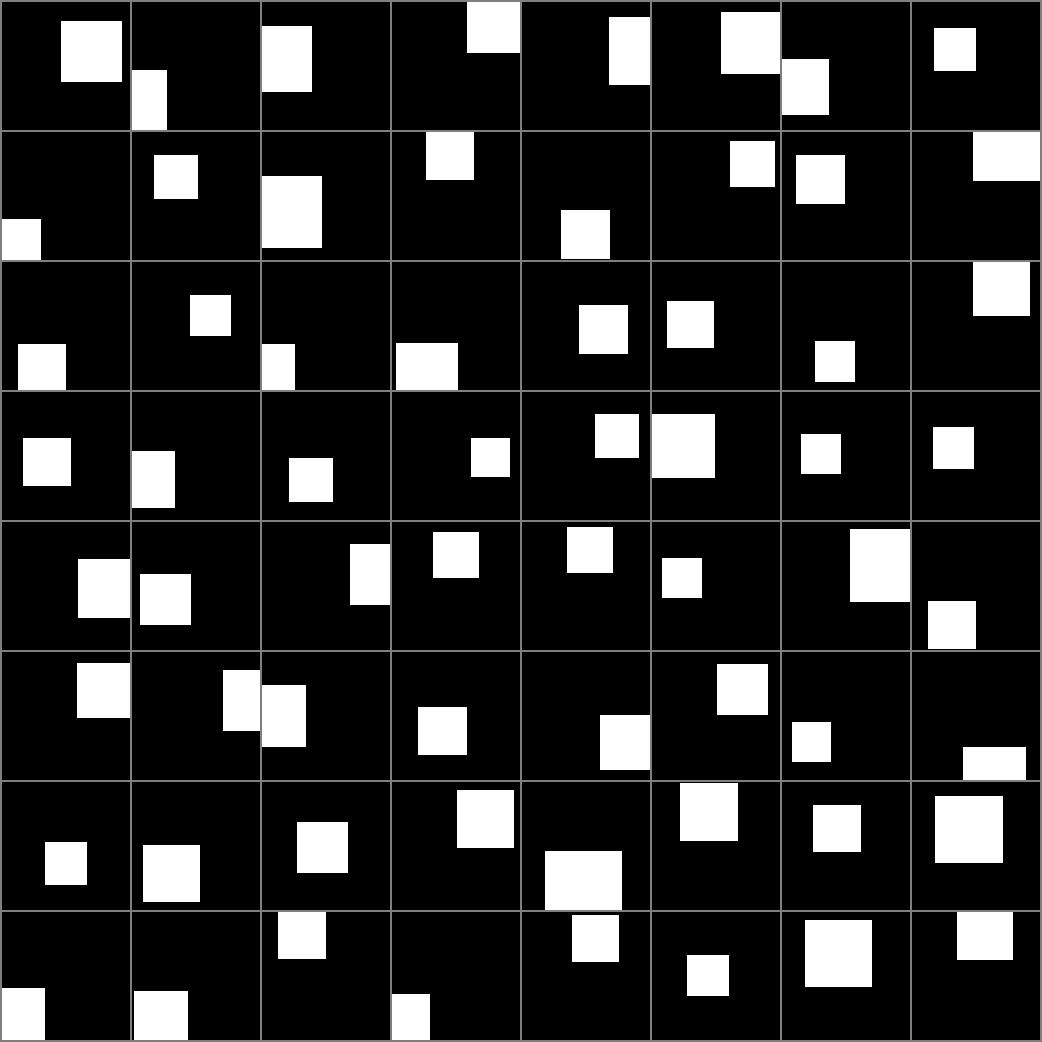
\includegraphics[width=\textwidth]{square_target1.png}
	\caption{Rotation target}
	\label{sq_rt}
\end{subfigure}
\caption{} \label{square_images}
\end{figure}



\begin{figure}[!ht]
\centering
\begin{subfigure}{0.3\textwidth}
	\centering
	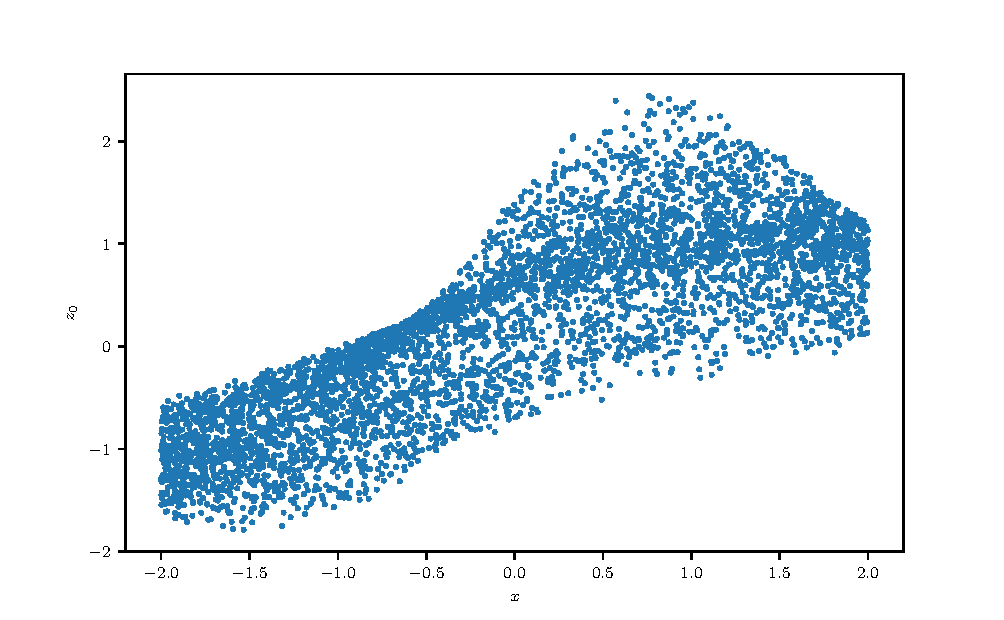
\includegraphics[width=\textwidth] {square_x_z0.pdf}
	\caption{}
	\label{fig_xzo}
\end{subfigure}
\begin{subfigure}{0.3\textwidth}
	\centering	
	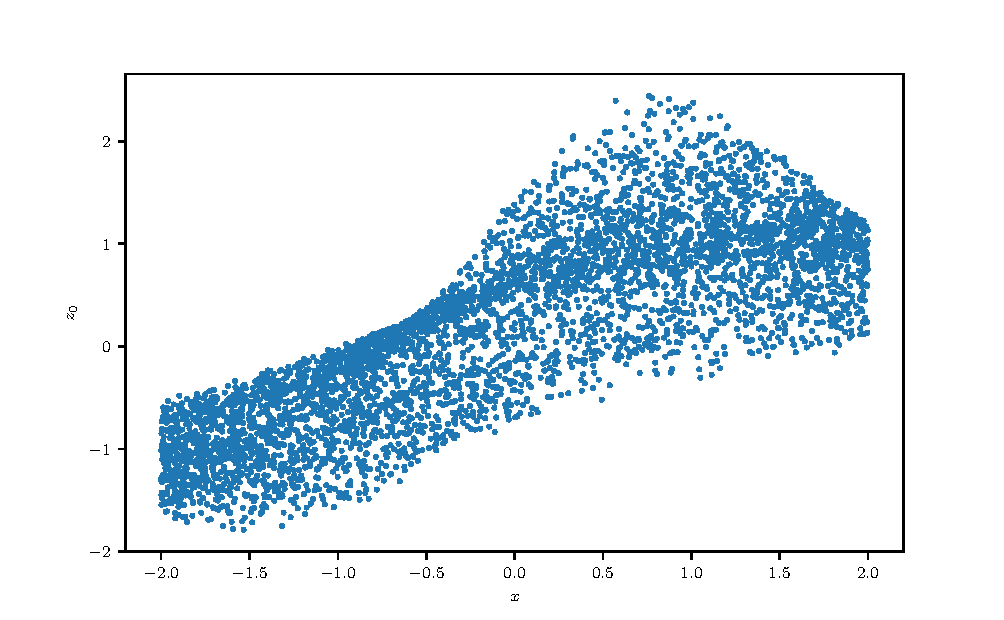
\includegraphics[width=\textwidth]{square_x_z0.pdf}
	\caption{}
	\label{fig_xz1}
\end{subfigure}
\begin{subfigure}{0.3\textwidth}
	\centering
	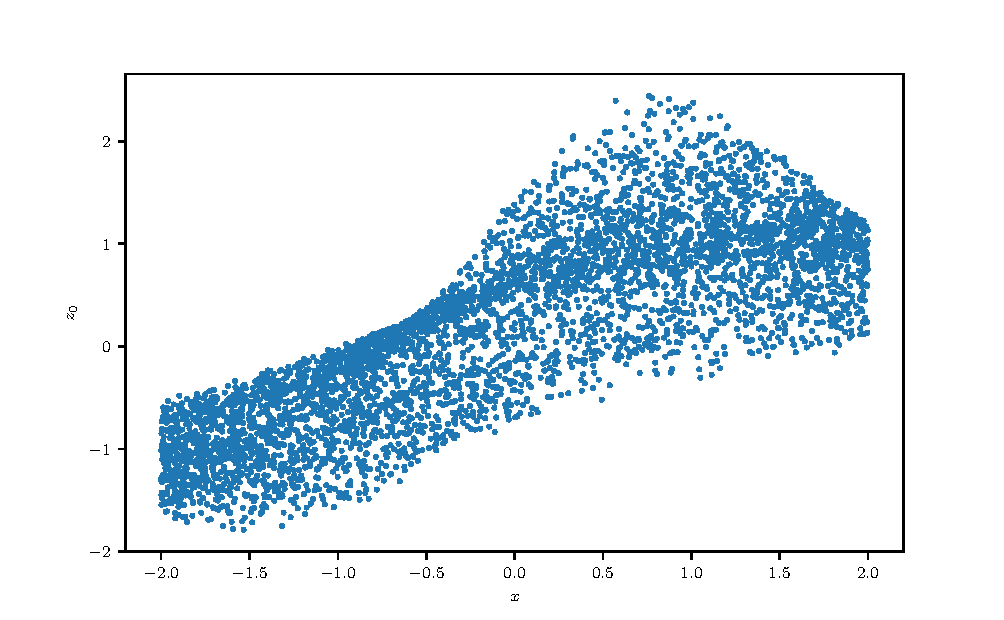
\includegraphics[width=\textwidth] {square_x_z0.pdf}
	\caption{}
	\label{fig_xz2}
\end{subfigure}
\begin{subfigure}{0.3\textwidth}
	\centering	
	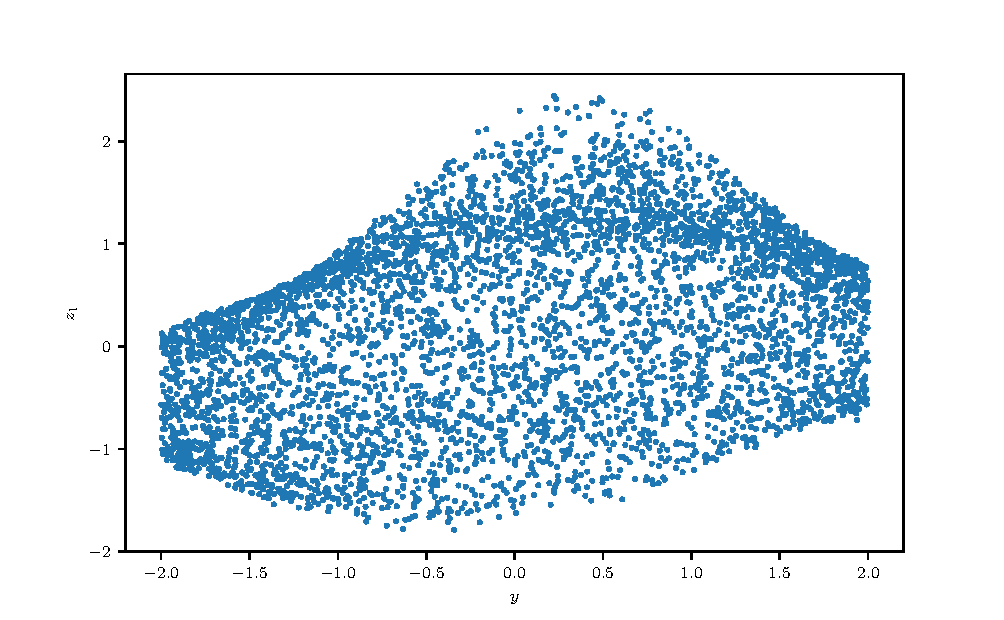
\includegraphics[width=\textwidth]{square_y_z1.pdf}
	\caption{}
	\label{fig_yz0}
\end{subfigure}
\begin{subfigure}{0.3\textwidth}
	\centering
	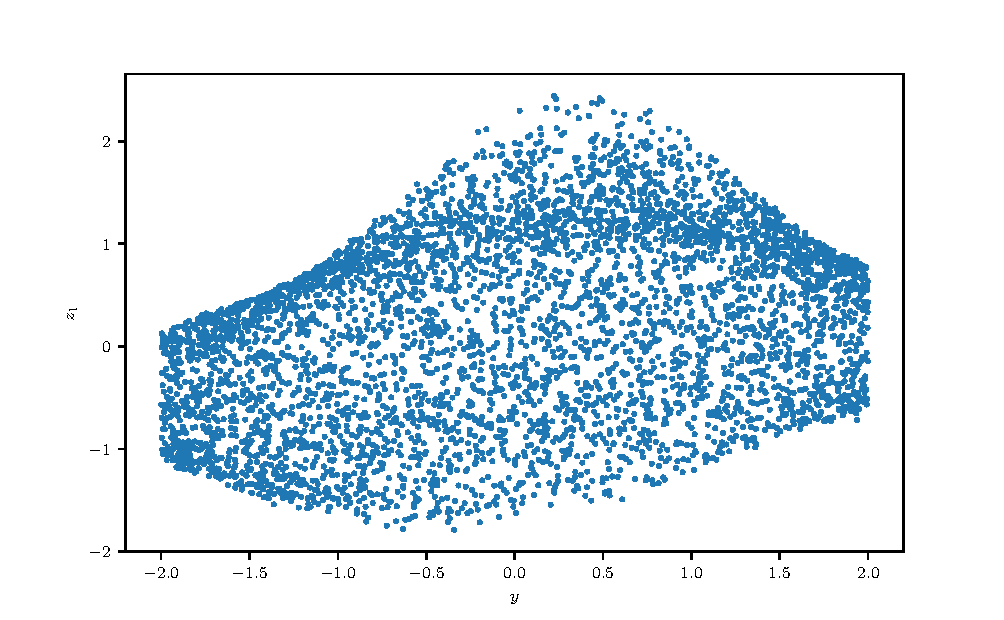
\includegraphics[width=\textwidth] {square_y_z1.pdf}
	\caption{}
	\label{fig_yz1}
\end{subfigure}
\begin{subfigure}{0.3\textwidth}
	\centering	
	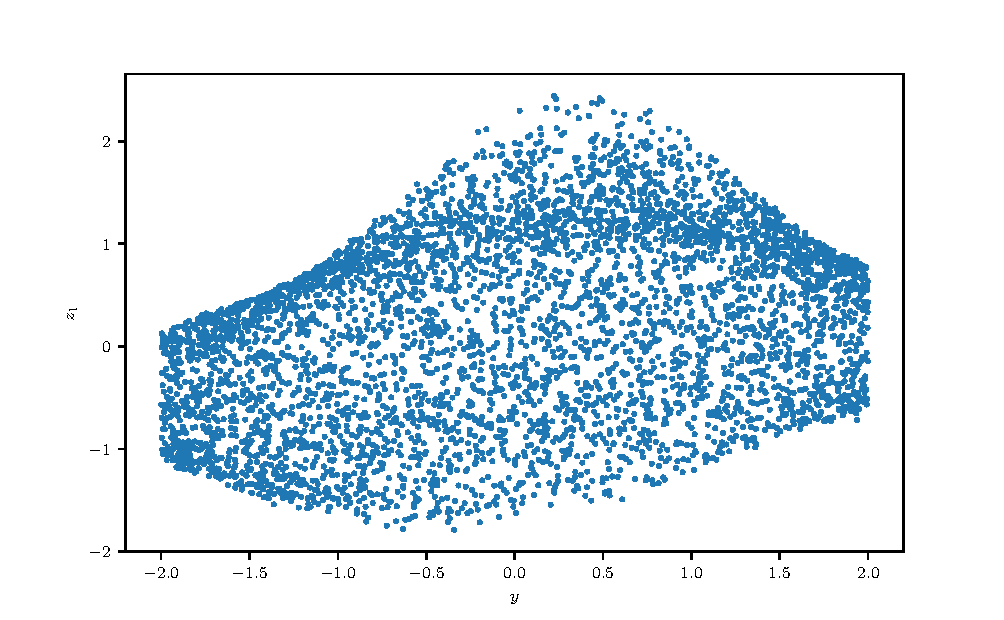
\includegraphics[width=\textwidth]{square_y_z1.pdf}
	\caption{}
	\label{fig_yz2}
\end{subfigure}
\begin{subfigure}{0.3\textwidth}
	\centering
	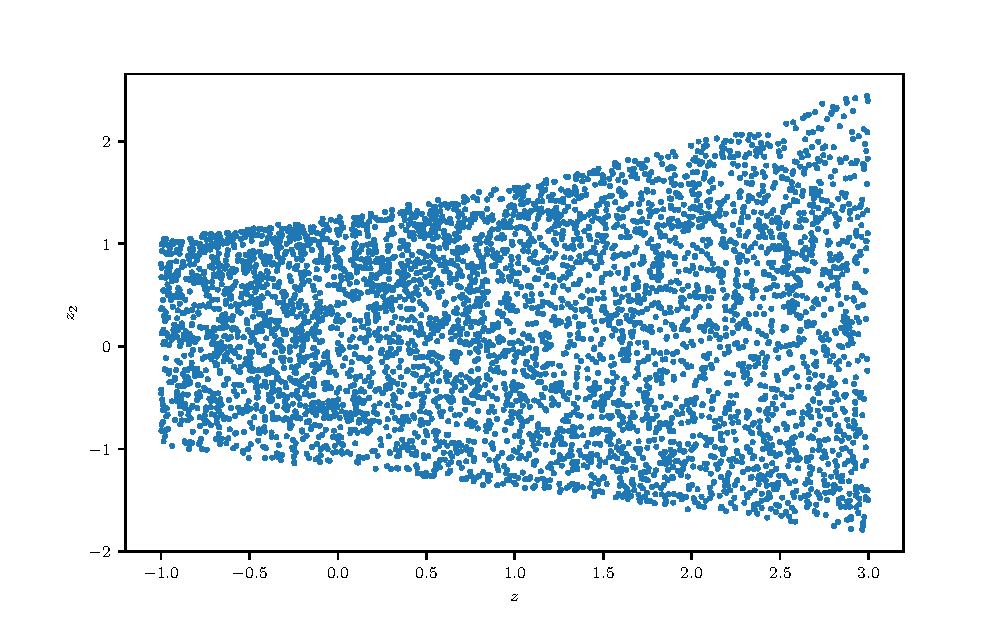
\includegraphics[width=\textwidth] {square_z_z2.pdf}
	\caption{}
	\label{fig_zzo}
\end{subfigure}
\begin{subfigure}{0.3\textwidth}
	\centering	
	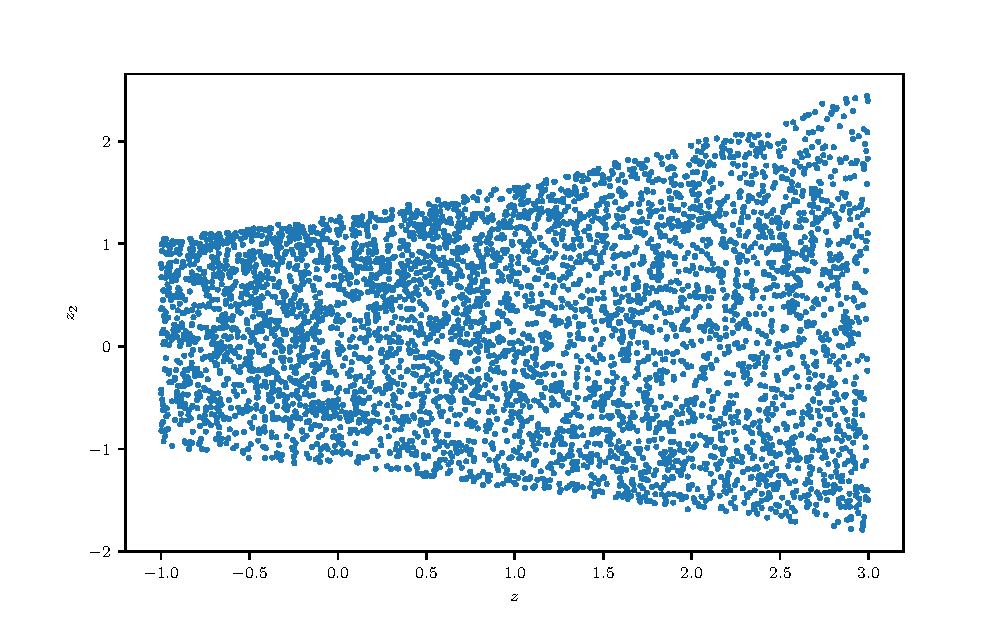
\includegraphics[width=\textwidth]{square_z_z2.pdf}
	\caption{}
	\label{fig_zz1}
\end{subfigure}
\begin{subfigure}{0.3\textwidth}
	\centering	
	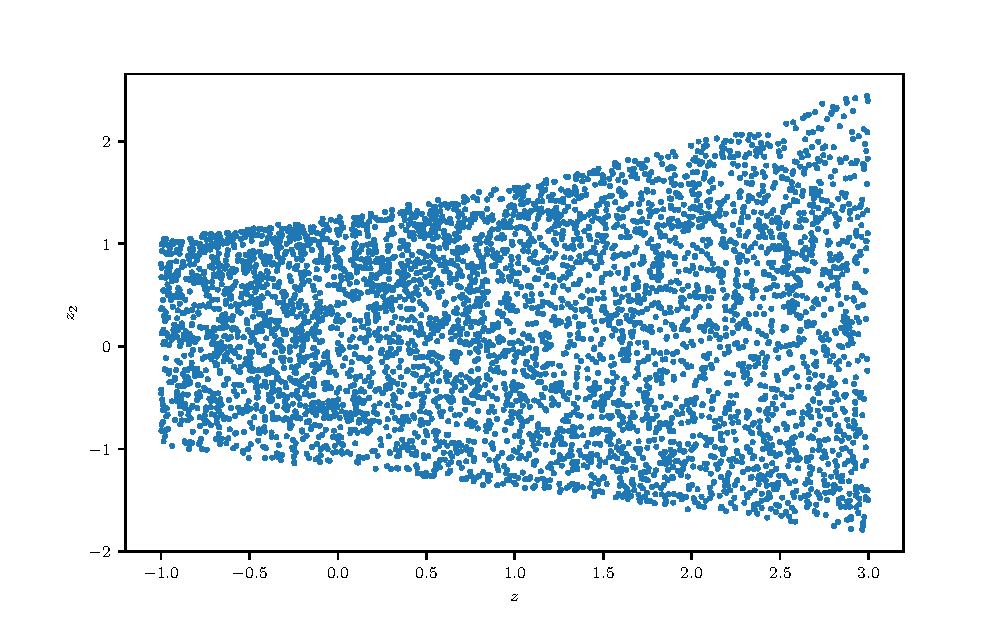
\includegraphics[width=\textwidth]{square_z_z2.pdf}
	\caption{}
	\label{fig_zz2}
\end{subfigure}
\caption{Correlation plots of the translations $x,y$ and $z$ and the dimensions of $z_{\rot}$ for the square.\\
The rows represent the translations in axes x,y and z e.g. (a-c) for x\\
The colums represent the $z_{\rot_i}$ e.g. (a), (d) and (g) for $z_{\rot_1}$} \label{Square_corr_trans}
\end{figure}


\begin{figure}[!ht]
\centering
\begin{subfigure}{\textwidth}
	\centering
	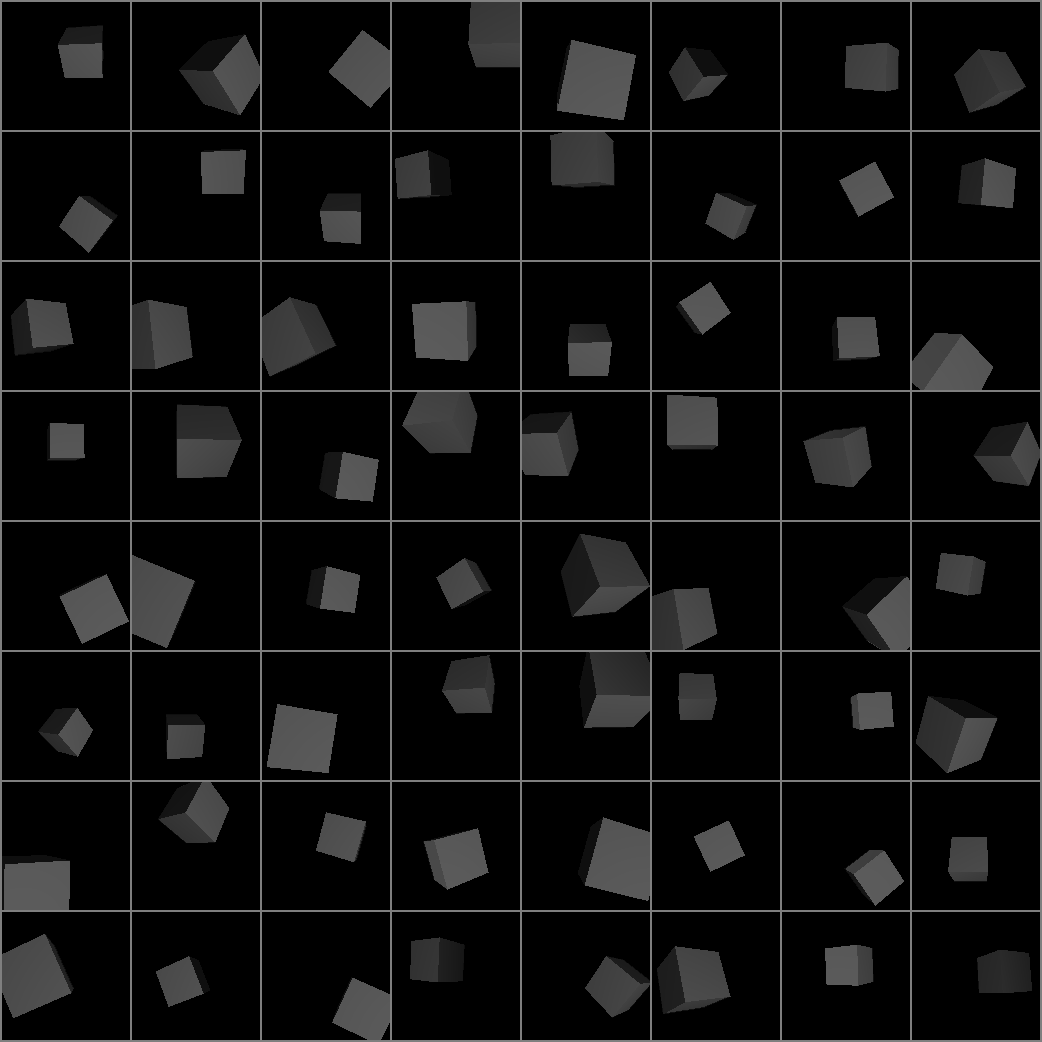
\includegraphics[width=0.49\textwidth] {cube_input.png}
	\caption{Input}
	\label{cube_in}
\end{subfigure}
\begin{subfigure}{0.49\textwidth}
	\centering
	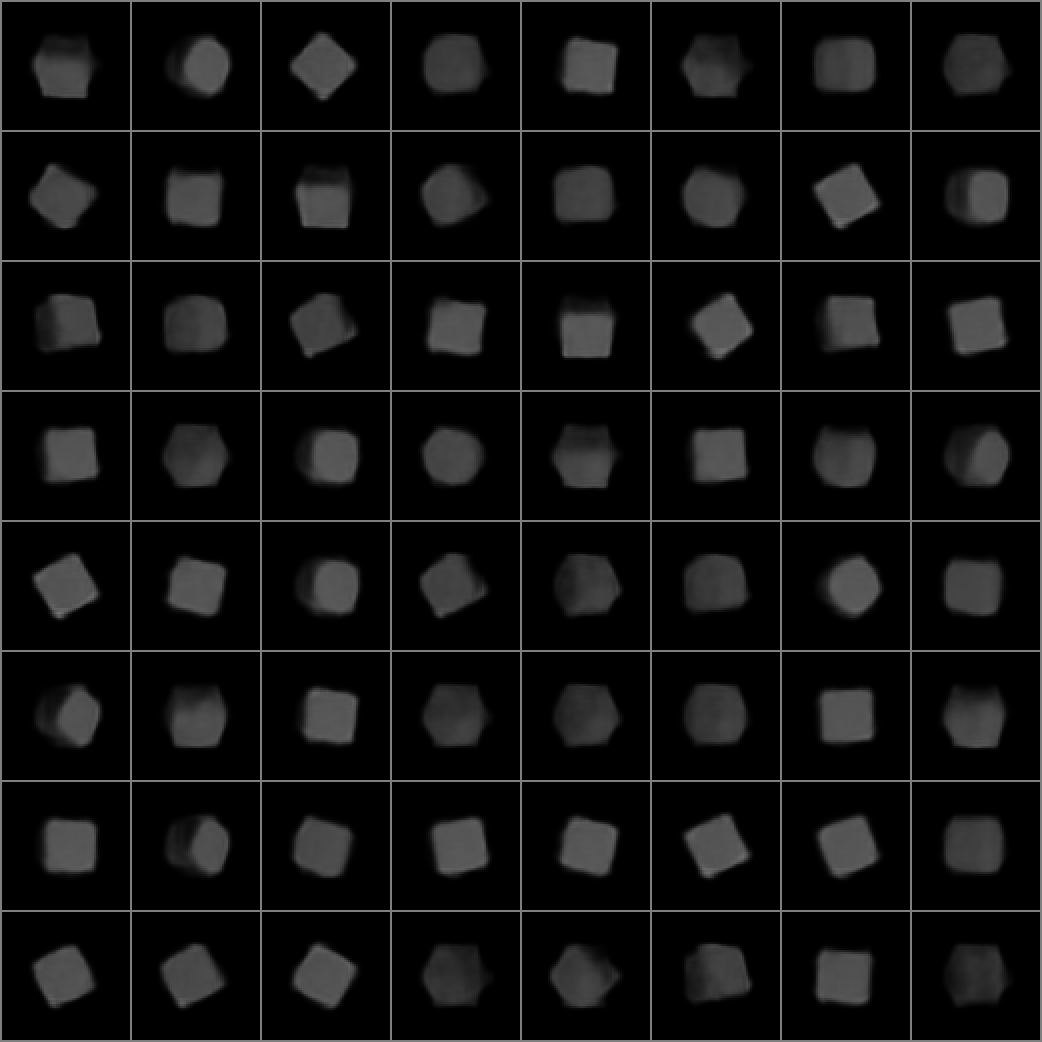
\includegraphics[width=\textwidth] {cube_output0.png}
	\caption{Translation reconstr.}
	\label{cube_trec}
\end{subfigure}
\begin{subfigure}{0.49\textwidth}
	\centering	
	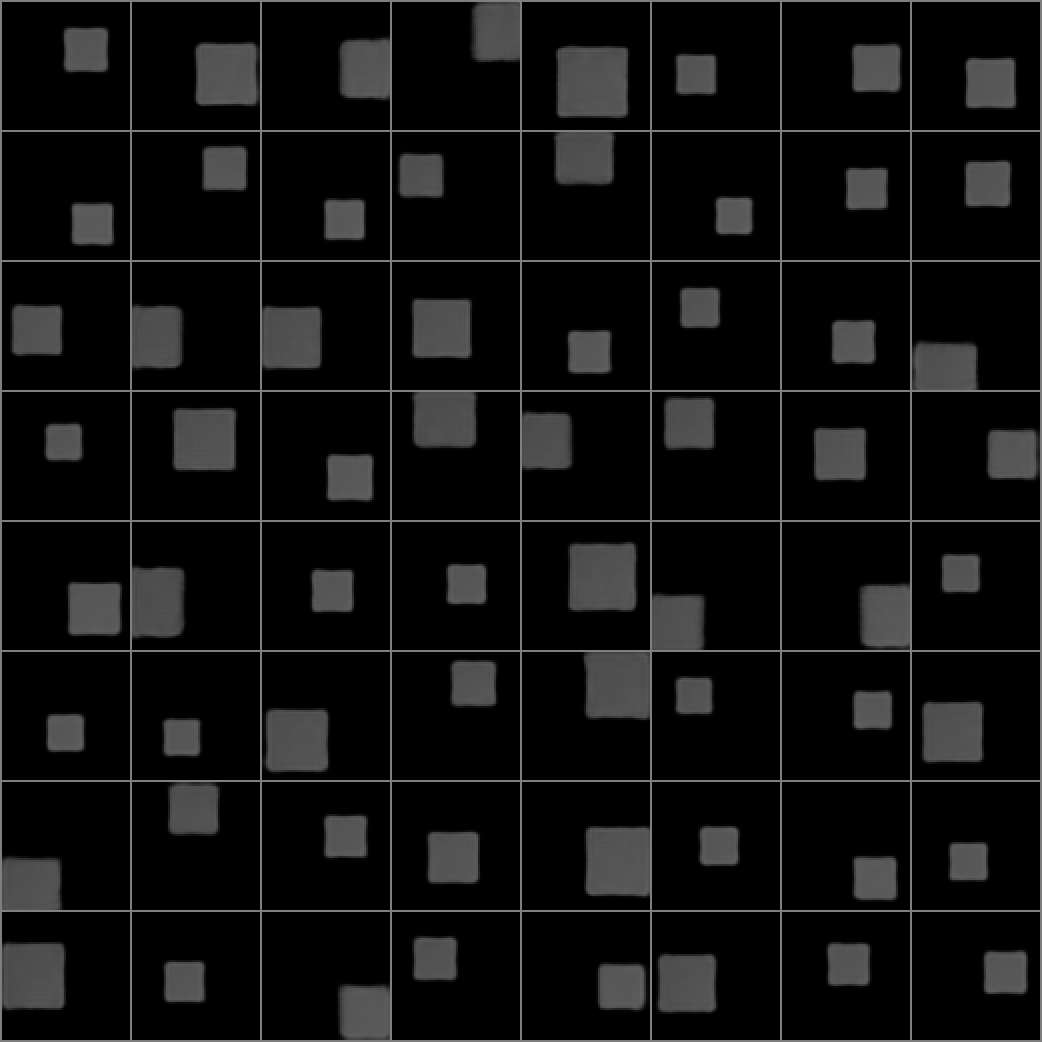
\includegraphics[width=\textwidth]{cube_output1.png}
	\caption{Rotation reconstr.}
	\label{cube_rrec}
\end{subfigure}
\begin{subfigure}{0.49\textwidth}
	\centering
	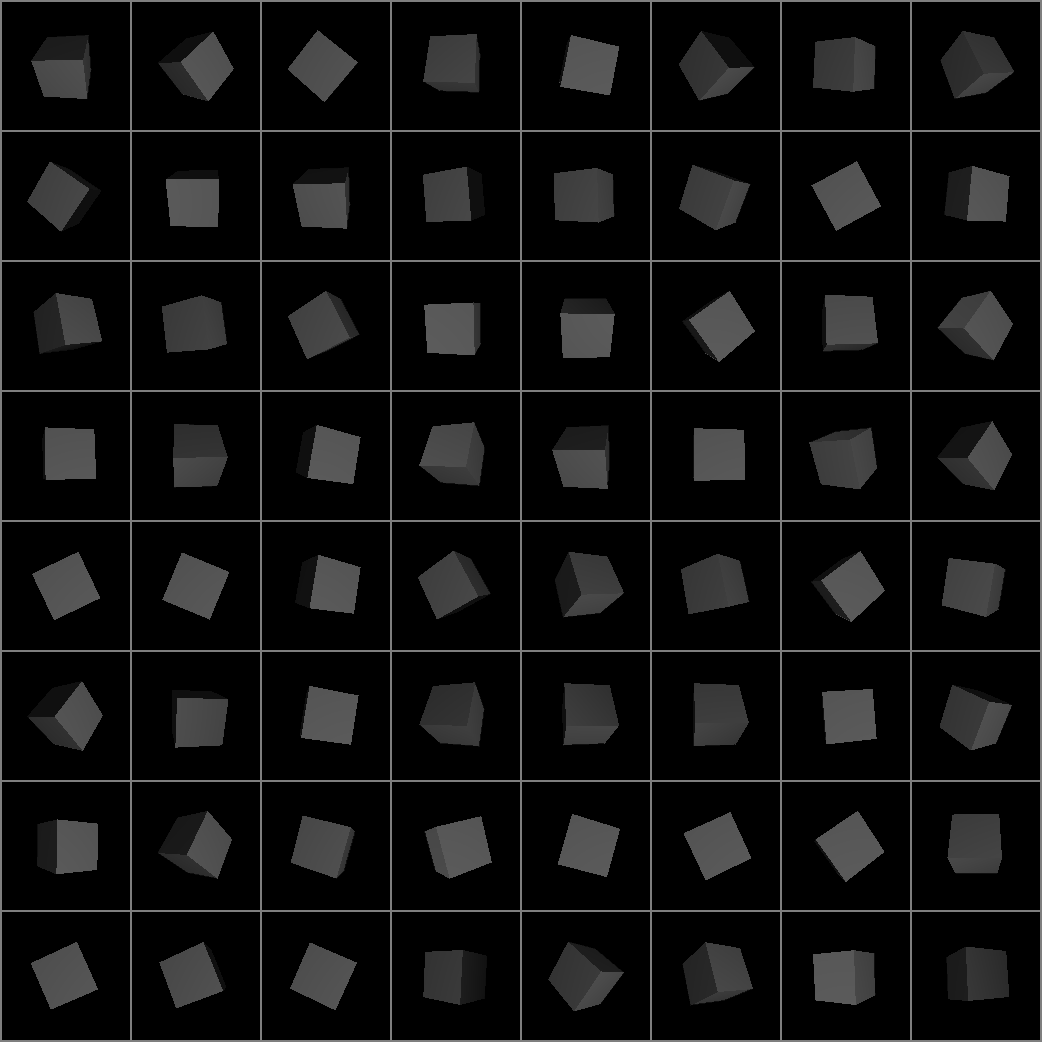
\includegraphics[width=\textwidth] {cube_target0.png}
	\caption{Translation target}
	\label{cube_tt}
\end{subfigure}
\begin{subfigure}{0.49\textwidth}
	\centering	
	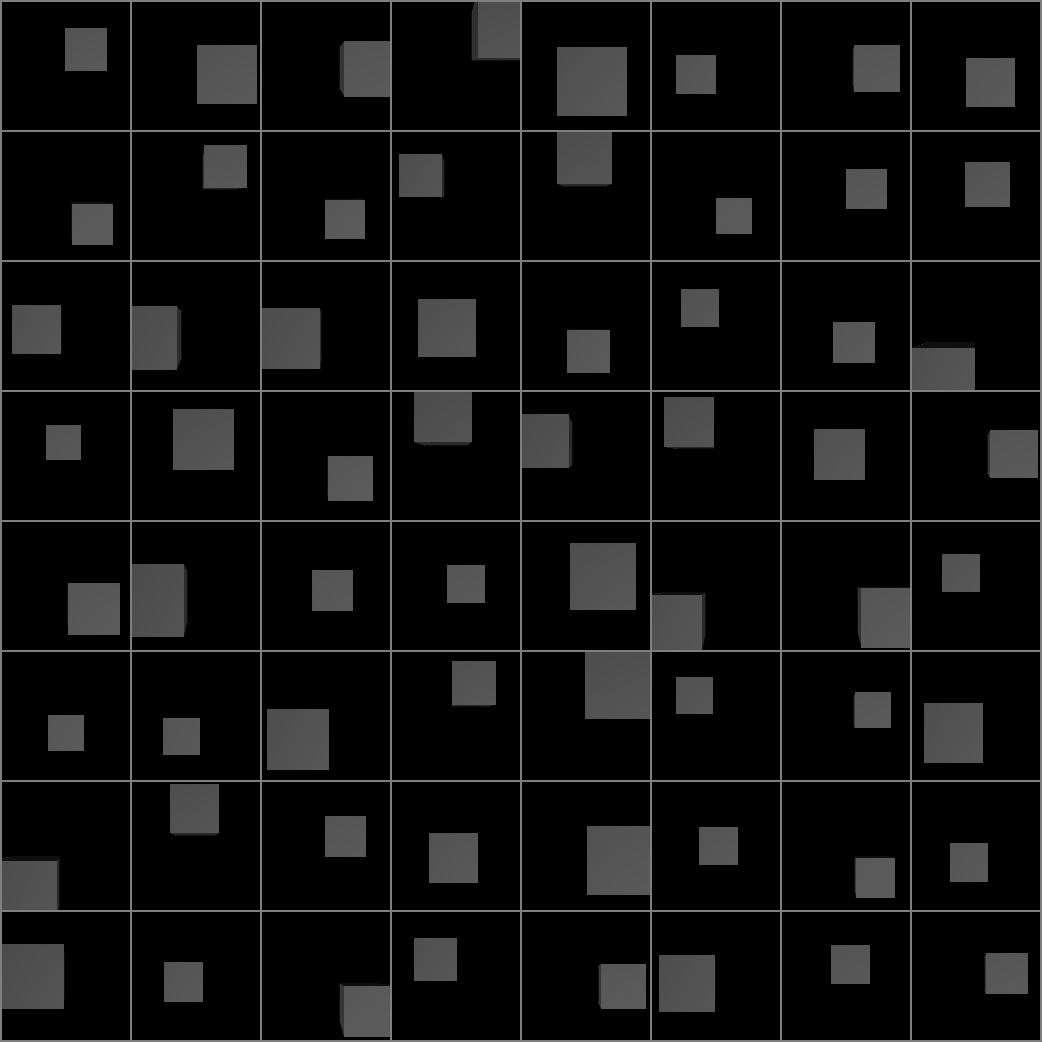
\includegraphics[width=\textwidth]{cube_target1.png}
	\caption{Rotation target}
	\label{cube_rt}
\end{subfigure}
\caption{} \label{cube_images}
\end{figure}



\begin{figure}[!ht]
\centering
\begin{subfigure}{0.3\textwidth}
	\centering
	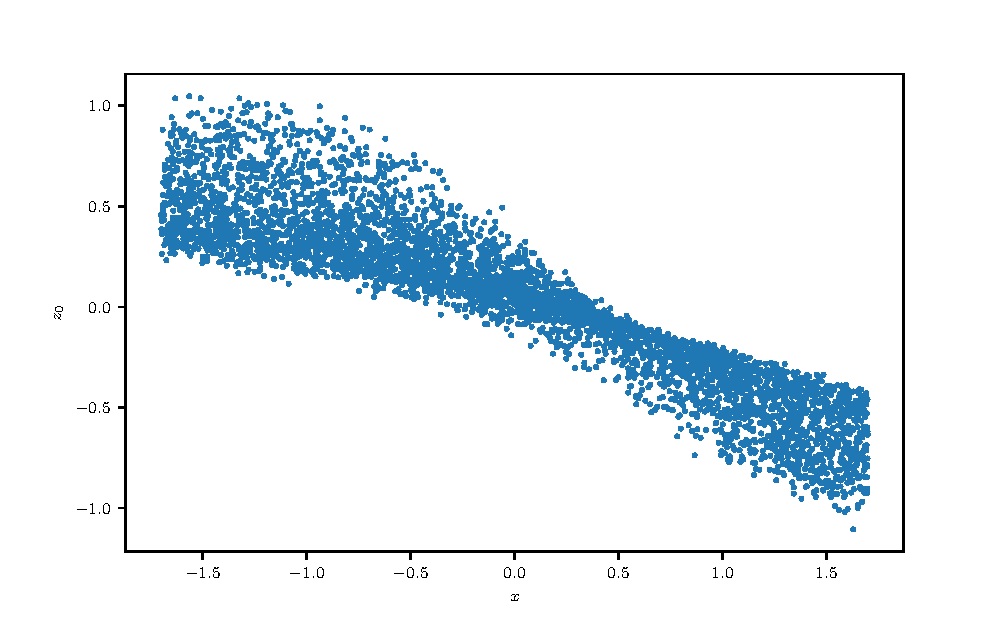
\includegraphics[width=\textwidth] {cube_trans_x_z0.pdf}
	\caption{}
	\label{cfig_xzo}
\end{subfigure}
\begin{subfigure}{0.3\textwidth}
	\centering	
	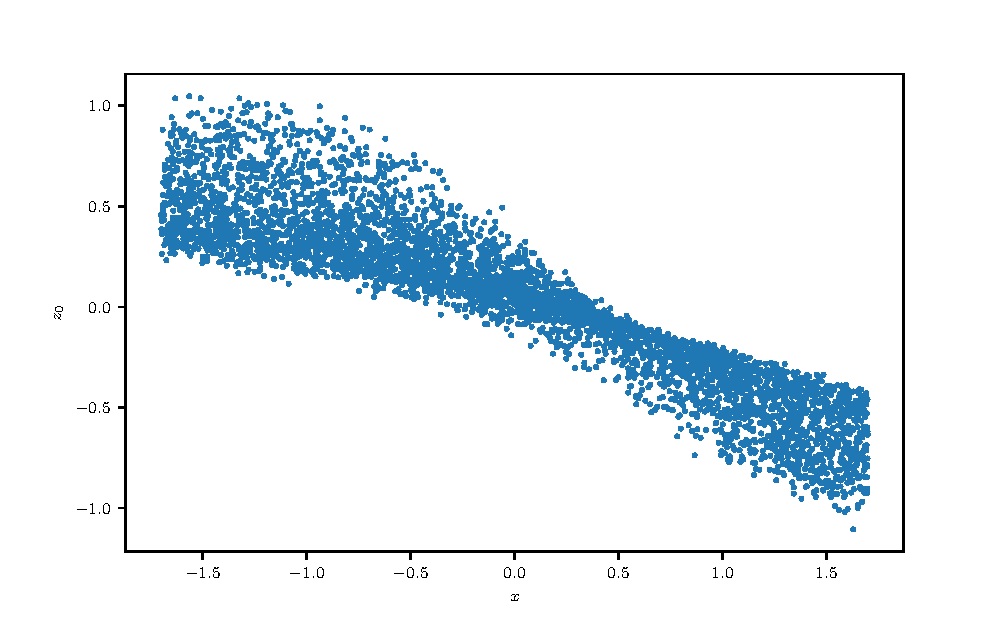
\includegraphics[width=\textwidth]{cube_trans_x_z0.pdf}
	\caption{}
	\label{cfig_xz1}
\end{subfigure}
\begin{subfigure}{0.3\textwidth}
	\centering
	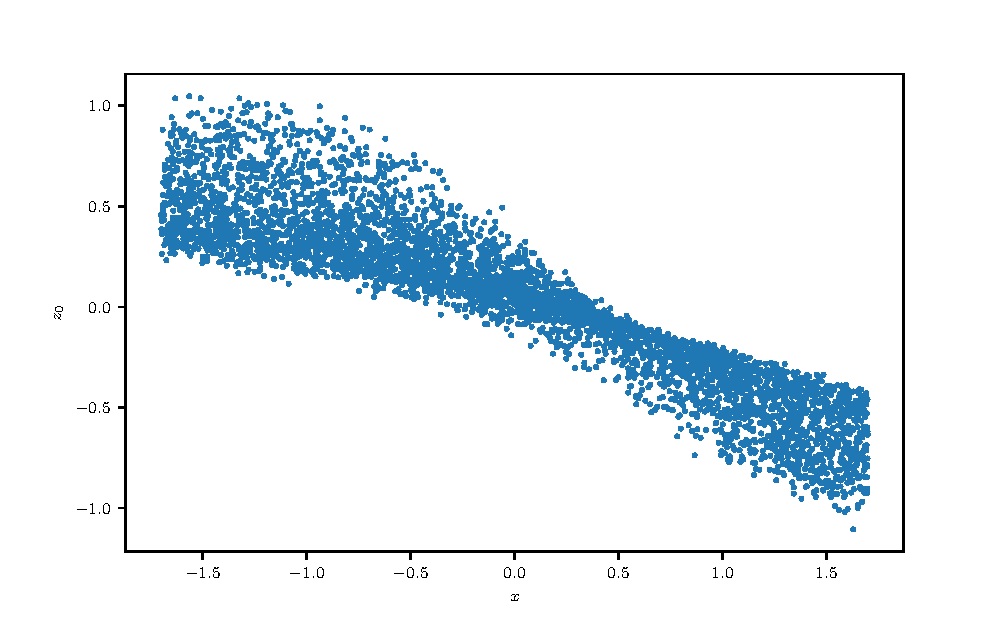
\includegraphics[width=\textwidth] {cube_trans_x_z0.pdf}
	\caption{}
	\label{cfig_xz2}
\end{subfigure}
\begin{subfigure}{0.3\textwidth}
	\centering	
	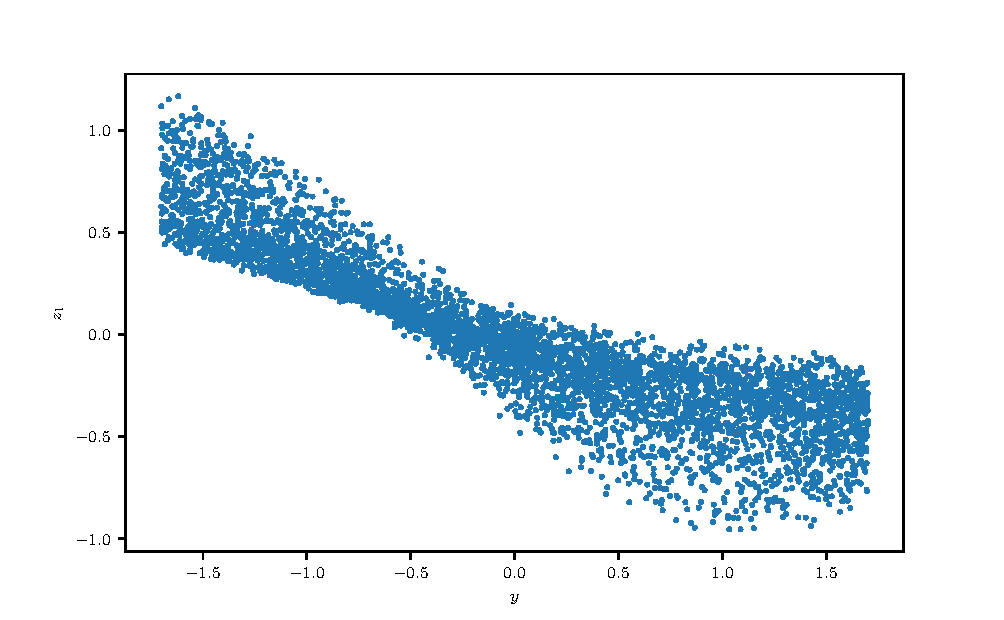
\includegraphics[width=\textwidth]{cube_trans_y_z1.pdf}
	\caption{}
	\label{cfig_yz0}
\end{subfigure}
\begin{subfigure}{0.3\textwidth}
	\centering
	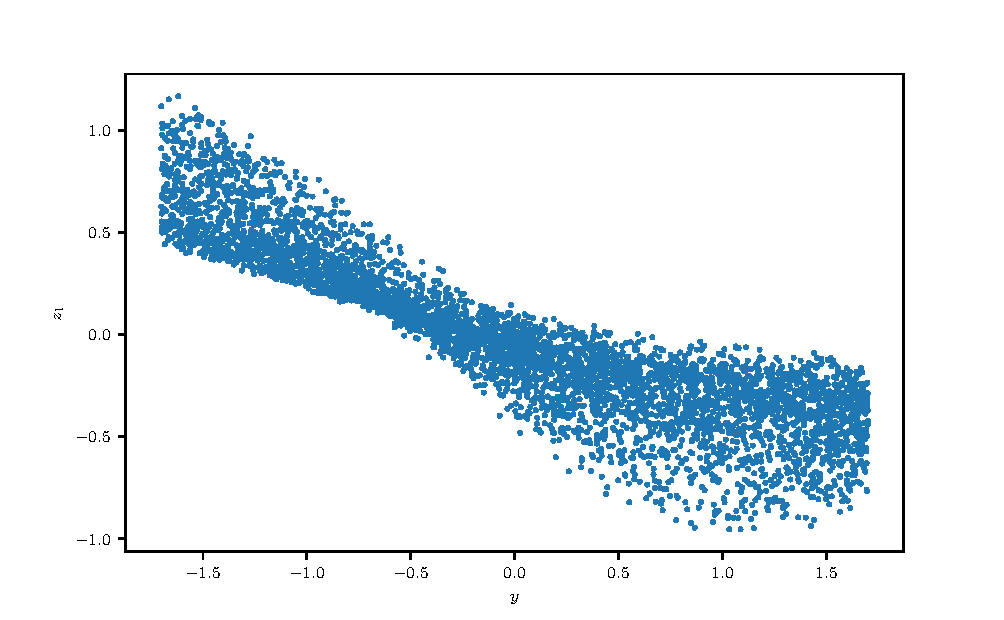
\includegraphics[width=\textwidth] {cube_trans_y_z1.pdf}
	\caption{}
	\label{cfig_yz1}
\end{subfigure}
\begin{subfigure}{0.3\textwidth}
	\centering	
	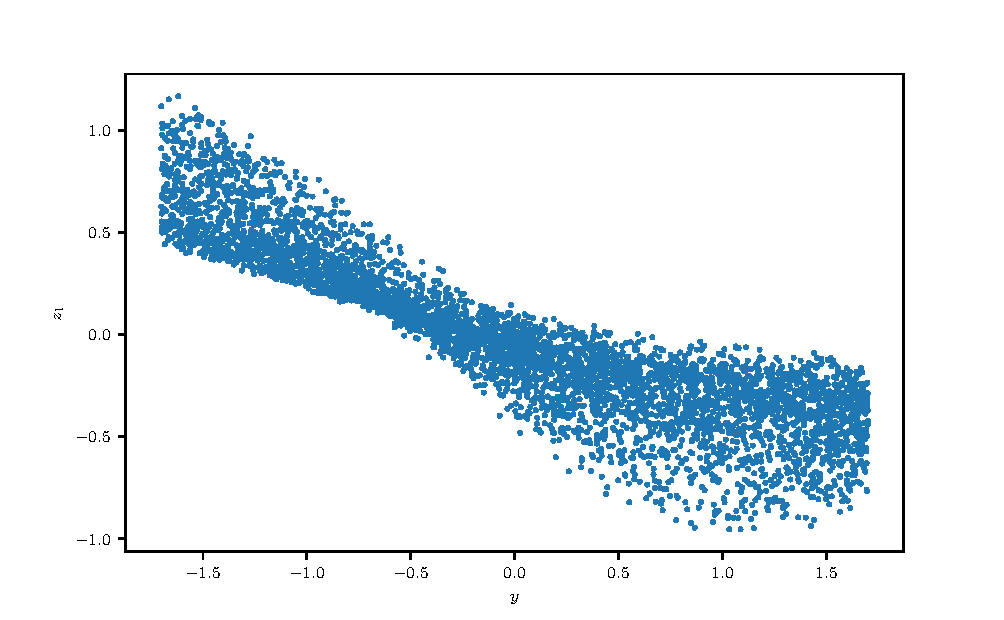
\includegraphics[width=\textwidth]{cube_trans_y_z1.pdf}
	\caption{}
	\label{cfig_yz2}
\end{subfigure}
\begin{subfigure}{0.3\textwidth}
	\centering
	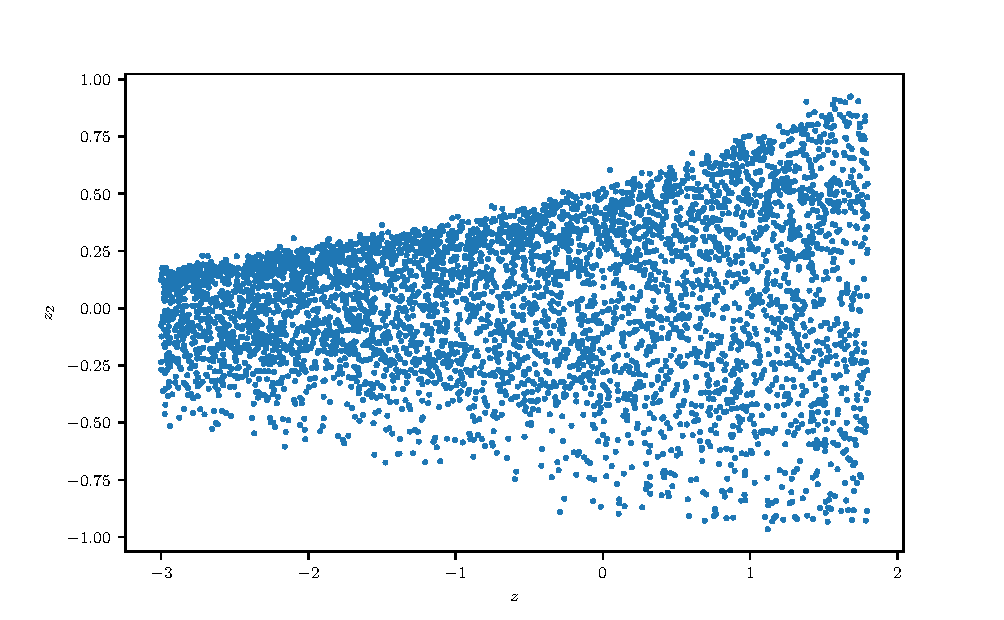
\includegraphics[width=\textwidth] {cube_trans_z_z2.pdf}
	\caption{}
	\label{cfig_zzo}
\end{subfigure}
\begin{subfigure}{0.3\textwidth}
	\centering	
	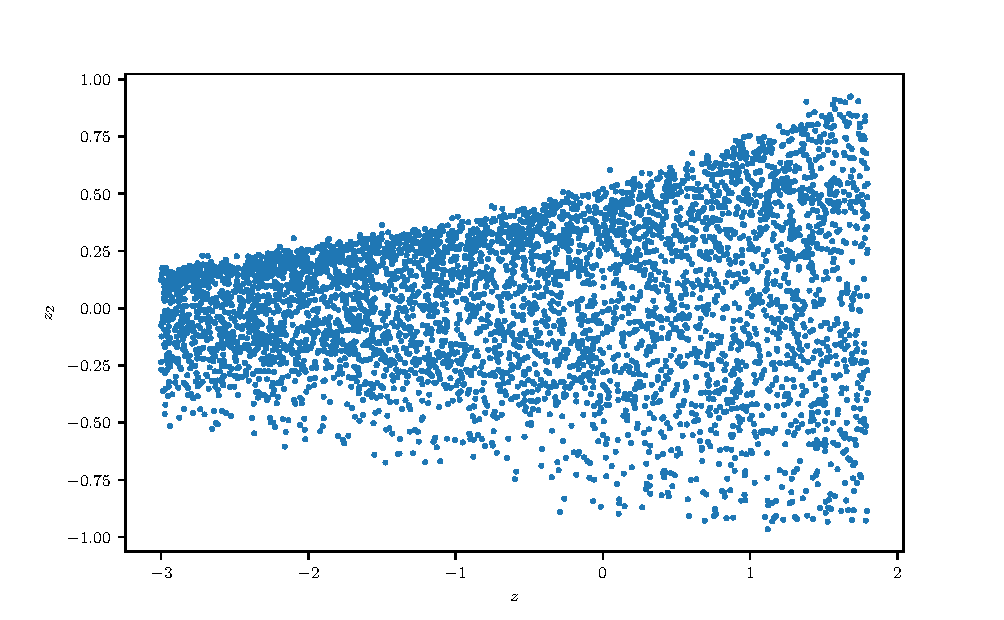
\includegraphics[width=\textwidth]{cube_trans_z_z2.pdf}
	\caption{}
	\label{cfig_zz1}
\end{subfigure}
\begin{subfigure}{0.3\textwidth}
	\centering	
	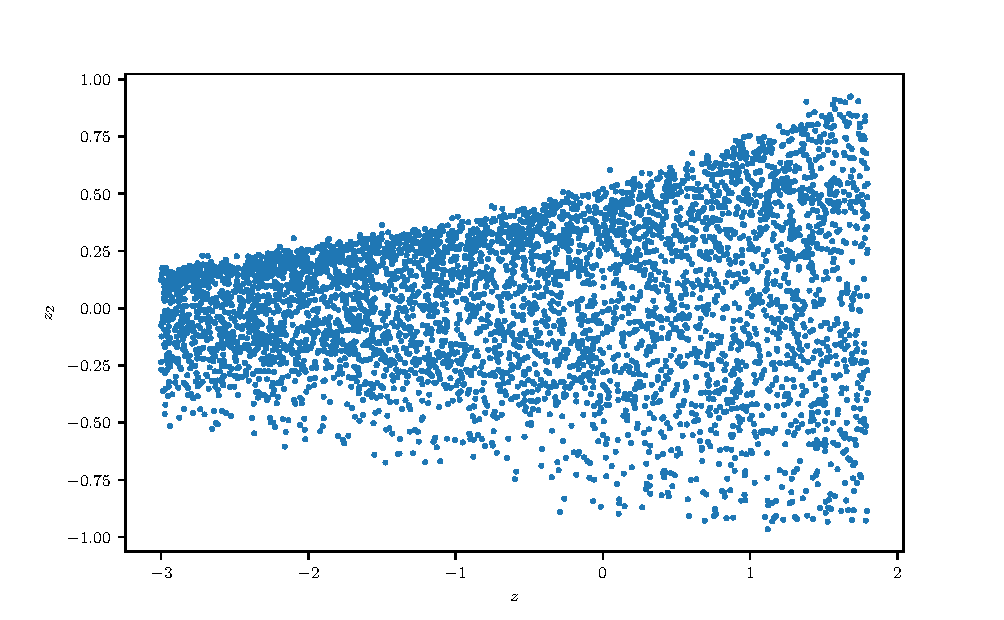
\includegraphics[width=\textwidth]{cube_trans_z_z2.pdf}
	\caption{}
	\label{cfig_zz2}
\end{subfigure}
\caption{Correlation plots of the translations $x,y$ and $z$ and the dimensions of $z_{\rot}$ for the cube.\\
The rows represent the translations in axes x,y and z e.g. (a-c) for x\\
The colums represent the $z_{\rot_i}$ e.g. (a), (d) and (g) for $z_{\rot_1}$} \label{cube_corr_trans}
\end{figure}


\end{document}
